%% Glaukopis -- Journal of Systems and Software (Elsevier) submission, v1.8 (2026-10-25).
%% Built from doc/v1.7 (Intl Journal of IS - Springer)/glaukopis_ijis.tex (the post-C&S revision expanded for
%% IJIS), re-framed for a software-engineering readership and ported to Elsevier's CAS double-column class
%% (cas-dc.cls 2.4, shipped in this folder). JSS review is single-anonymized, so author names stay in.
%% Build: bash build.sh  (pdflatex -> bibtex -> pdflatex x2); needs cas-dc.cls, cas-common.sty and
%% cas-model2-names.bst next to this file. Highlights are not typeset in the PDF; upload highlights.txt.
%% Before submitting, search for "TODO (authors)".
\documentclass[a4paper,fleqn]{cas-dc}
\usepackage[authoryear]{natbib}
\usepackage{tabularx}
\renewcommand{\tabularxcolumn}[1]{>{\raggedright\arraybackslash}p{#1}}
\newcolumntype{P}[1]{>{\raggedright\arraybackslash}p{#1}}
\usepackage{xurl}
\usepackage{tikz}
\usetikzlibrary{arrows.meta,positioning,fit,backgrounds,calc}
\usepackage{pgfplots}
\usepgfplotslibrary{groupplots}
\pgfplotsset{compat=1.15}
\usepackage{listings}
\setlength{\emergencystretch}{2em}
\renewcommand{\topfraction}{0.95}
\renewcommand{\bottomfraction}{0.95}
\renewcommand{\textfraction}{0.03}
\renewcommand{\floatpagefraction}{0.75}
\setcounter{topnumber}{4}\setcounter{bottomnumber}{4}\setcounter{totalnumber}{8}\setcounter{dbltopnumber}{4}
\lstset{basicstyle=\footnotesize\ttfamily,breaklines=true,columns=fullflexible,keepspaces=true,frame=single,showstringspaces=false}
\newcommand{\code}[1]{\path{#1}}
\newsavebox{\fitbox}
\newcommand{\fitwidth}[1]{\sbox{\fitbox}{#1}\ifdim\wd\fitbox>\textwidth\resizebox{\textwidth}{!}{\usebox{\fitbox}}\else\usebox{\fitbox}\fi}
\newcommand{\ci}[2]{{\scriptsize[#1,\,#2]}}
\newcommand{\Abal}{A_{\mathrm{bal}}}
\newcommand{\Bbal}{B_{\mathrm{bal}}}
\newcommand{\Tbal}{T_{\mathrm{bal}}}
\definecolor{seriesblue}{HTML}{2A78D6}
\definecolor{refgray}{HTML}{52514E}

\begin{document}
\let\WriteBookmarks\relax
\def\floatpagepagefraction{1}
\def\textpagefraction{.001}

\shorttitle{Layered instruction fine-tuning for CTI LLM training}
\shortauthors{P. J. Worth Jr. and I. Cardei}

\title[mode=title]{Glaukopis: Layered Instruction Fine-Tuning for Cyber Threat Intelligence LLM Training}

\author[1,2]{Peter J. Worth Jr.}[orcid=0000-0003-4211-3866]
\cormark[1]
\ead{pworthjr@athenasecuritygrp.com}
\credit{Conceptualization, Methodology, Software, Investigation, Data curation, Formal analysis, Writing -- original draft, Writing -- review and editing}

\author[1,2]{Ionut Cardei}[orcid=0009-0000-1050-768X]
\credit{Supervision, Methodology, Writing -- review and editing}

\affiliation[1]{organization={Department of Electrical Engineering and Computer Science, Florida Atlantic University},
  addressline={777 Glades Road}, city={Boca Raton}, state={FL}, postcode={33431}, country={USA}}
\affiliation[2]{organization={Athena Software Group Inc.},
  addressline={294 Queens Ct}, city={West Palm Beach}, state={FL}, postcode={33401}, country={USA}}

\cortext[1]{Corresponding author}

\begin{abstract}
Organizations that cannot send security data to hosted services increasingly specialize open-weight language models for cyber threat intelligence (CTI): mapping vulnerabilities to weakness classes, extracting attack techniques, recommending mitigations, and attributing intrusions. Building such a model is a software-engineering problem: its developers must know where each training example came from, which data defects the pipeline's checks catch, and where in a multi-stage training pipeline a capability was gained or lost. We report Glaukopis, a pipeline that generates instruction-tuning data by executing typed queries over a knowledge graph of twelve public CTI sources, so that every CTI training target resolves to the graph facts that produced it, and that fine-tunes Qwen2.5-32B-Instruct in four layered stages while retaining and evaluating each stage's checkpoint. The evaluation uses three CTI benchmarks and a general-reasoning diagnostic, compares against the base model, a security-specialized open model, six hosted frontier models, and a single-stage baseline, and reports item-level bootstrap intervals and response-level error taxonomies. The final checkpoint raises the three-benchmark mean from 57.7 to 65.0, but the gain is confined to the benchmark whose task schemas the data targets; two independently built benchmarks are unchanged and general reasoning falls by 11.6 points. Against the single-stage baseline formed by the first stage's checkpoint, the three later stages add 3.2 points to the three-benchmark mean but cost 2.3 on the aligned benchmark; checkpoint-level analysis traces that cost, an attribution collapse, and a severity regression to one stage of short structured-answer drills. Seven lessons for practice conclude the article.
\end{abstract}

\begin{keywords}
Software engineering for AI \sep Instruction fine-tuning \sep Training-data provenance \sep Knowledge graphs \sep Cyber threat intelligence \sep Capability regression \sep Language-model evaluation
\end{keywords}

\maketitle

\section{Introduction}\label{sec:intro}
Cyber threat intelligence (CTI) is the practice of collecting, structuring, and acting on knowledge about adversaries, their techniques, and the vulnerabilities they exploit. Much of that knowledge is published as public catalogs with stable identifiers: the MITRE ATT\&CK matrix of adversary techniques (T-codes) and groups (G-codes), the Common Weakness Enumeration (CWE), the Common Vulnerabilities and Exposures list (CVE) with its CVSS severity vectors, and detection and mitigation catalogs built around them. A security analyst's routine work consists largely of mapping between these catalogs under time pressure: deciding which weakness class explains a new vulnerability description, which ATT\&CK technique an observed behavior corresponds to, which mitigations apply to a technique, and which known actor an intrusion resembles. These are exactly the tasks that recent CTI benchmarks such as CTIBench and AthenaBench measure, because a general language model can be fluent and still return a parent technique instead of the requested sub-technique, a related but wrong CWE, or a malformed structured answer \citep{alam2024ctibench,alam2025athenabench}.

Many security operations centers (SOCs) would like to use a language model for this work but cannot send incident data to a hosted service because of contractual, confidentiality, or data-residency constraints. The practical option is to take an open-weight model, specialize it on CTI data, and serve it locally. The specialized model is then a software artifact produced by a pipeline of data generation, filtering, training, and evaluation, and it inherits the quality problems that software-engineering research has documented for machine-learning systems: undeclared data dependencies, data defects that no compiler catches, and changes whose effects are entangled \citep{sculley2015hidden,amershi2019se4ml,martinez2022se4ai}. Two of these problems are acute for instruction-tuned models. The first is the traceability of the training data: when instruction-tuning examples are synthesized (by a model, by annotators, or by templates), can a reviewer trace a given training target back to the public fact that justifies it, and does the pipeline detect a defective example before it is trained on? The second is the localization of regressions: a single aggregate score for the final model does not say which capabilities improved, which regressed, and which step of the pipeline introduced the regression.

Glaukopis is the framework we built to answer both questions; its components are named after figures from Greek mythology and are introduced here once. \emph{Ariadne} is a knowledge graph, stored in Neo4j, that integrates twelve public CTI sources (Section~\ref{sec:data}). \emph{Sophia} is a template engine that produces an instruction-tuning example by executing a typed query against Ariadne and rendering the returned graph binding into an instruction, an optional context, and a target answer; the target is therefore a deterministic function of specific graph facts, and every CTI example in the corpus carries the identifier of the template that produced it. The training recipe fine-tunes Qwen2.5-32B-Instruct, a 32-billion-parameter open-weight model that fits on two 80-GB GPUs for serving, in four supervised stages, each layered on the checkpoint of the stage before it, and keeps every stage's checkpoint. Evaluating every retained checkpoint on the same benchmark suite turns training into a sequence of observable transitions, which is what allows us to locate when a capability is lost and to inspect the responses that lost it.

The evaluation must be read with two facts in mind, both of which bear on independence. First, the training templates deliberately cover the task schemas that the AthenaBench benchmark tests, because those schemas are the operational tasks the model is meant to perform. Second, AthenaBench was created by a team that includes one of the present authors (Worth). The training data and the benchmark items were built by different pipelines from different inputs, and we quantify their overlap at the level of 13-grams, entities, and gold facts (Section~\ref{sec:overlap}). But the people who designed the benchmark also designed the training templates, and that shared knowledge of the task schemas is a form of alignment that no overlap measurement removes. We therefore treat AthenaBench as the aligned, in-domain benchmark and rely on two benchmarks built by unrelated groups (CyberSOCEval and CyberMetric) and on a general-reasoning diagnostic (MMLU-Pro) as the independent evidence. On that evidence the final checkpoint does not improve over the base model, and on MMLU-Pro it loses 11.6 points.

The study is organized around five research questions.
\begin{description}
\item[RQ1 (traceability and validation).] Does graph-materialized generation make every CTI training target traceable to the facts that produced it, and which data defects do the pipeline's checks catch and miss?
\item[RQ2 (gains and costs).] What does specialization gain on the aligned benchmark, and what does it gain or lose on independently built CTI benchmarks and on general reasoning, relative to the base model, a security-specialized open model, and hosted frontier models?
\item[RQ3 (localization).] At which stage are the gains and the regressions introduced, and what in the training data explains them?
\item[RQ4 (staging).] What do the later stages add to, and take from, the single-stage model that the first stage produces?
\item[RQ5 (evaluation validity).] How much of the gain can overlap between the training data and the benchmark items explain?
\end{description}

The contributions are: (i) a CTI data-generation pipeline in which every training target resolves to an executed graph query over public-source identifiers, with an account of the defects its checks catch and miss; (ii) a retained-checkpoint protocol for diagnosing capability regressions, with item-level uncertainty, response-level error taxonomies, and a mechanistic account of the two regressions observed; (iii) a quantified audit of training--evaluation overlap at the $n$-gram, entity, and gold-fact levels; (iv) an evaluation against the base model, a security-specialized open model, six hosted frontier models, and the single-stage baseline formed by the pipeline's first stage, with explicit statements of what each comparison does and does not control; and (v) lessons for engineering domain-specialized models, drawn from the release and its predecessors. The software is source-available \citep{glaukopis2026software}.

The results should be read accordingly. Glaukopis demonstrates a traceable way to construct CTI instruction data and a diagnostic protocol that shows what a specialization recipe gives and takes away. The four-stage schedule is measured against its own first stage, a single-stage fine-tune on the core shards that serves as the study's single-stage baseline (Section~\ref{sec:singlestage}): the three later stages add 3.2 points to the three-benchmark mean and cost the aligned benchmark 2.3, so staging is reported as a trade with a measured price, not as a uniform improvement.

The rest of the article is organized as follows. Section~\ref{sec:overview} gives an overview of the system and defines the names and acronyms used throughout. Section~\ref{sec:problem} states the problem. Section~\ref{sec:related} reviews related work. Sections~\ref{sec:data} and~\ref{sec:training} describe the data pipeline and the training recipe, including the single-stage baseline. Section~\ref{sec:evaluation} describes the benchmarks, baselines, aggregation conventions, overlap audit, and uncertainty estimates. Section~\ref{sec:results} reports and interprets the results, and Section~\ref{sec:cost} reports inference efficiency. Section~\ref{sec:discussion} answers the research questions and draws lessons for practice, Section~\ref{sec:limits} discusses threats to validity, Section~\ref{sec:directions} lists research directions, and Section~\ref{sec:conclusion} concludes. The supplementary material describes the evaluation suites (Section~S1) and the contamination screen (Section~S2) and gives one verbatim training record per template family (Section~S3).

\section{System overview and terminology}\label{sec:overview}
Figure~\ref{fig:pipeline} shows the three parts of the system as configured for the release evaluated here (internally, release v21). Public CTI sources are loaded into Ariadne; Sophia executes templates against Ariadne to produce four training shards; the shards are used in four stages of supervised fine-tuning; and every retained checkpoint is evaluated on the same suite. Table~\ref{tab:glossary} defines the names that recur in the article. Two conventions apply throughout. A \emph{shard} is a serialized training file produced by one Sophia run; a \emph{stage} is one fine-tuning pass that consumes one or more shards and starts from the checkpoint of the previous stage. Checkpoints are named after the stage that produced them (Core, +TAA, CSE, Recal-32B), and ``base'' denotes the unmodified Qwen2.5-32B-Instruct model.

\begin{table*}
\centering\footnotesize
\caption{Names and acronyms used in this article.}\label{tab:glossary}
\begin{tabularx}{\textwidth}{@{}P{3.2cm}X@{}}
\toprule Term & Meaning \\\midrule
Glaukopis & The framework as a whole: graph, template engine, training recipe, evaluation harness. \\
Ariadne & The Neo4j knowledge graph that integrates twelve public CTI sources (Section~\ref{sec:data}). \\
Sophia & The template engine that executes typed graph queries against Ariadne and renders the bindings into instruction-tuning records. \\
Core-A, Core-B & The two Sophia shards used in Stage 1: Core-A covers broad CTI knowledge and question formats; Core-B covers the four catalog-mapping schemas (mitigation, technique extraction, severity, root cause). \\
TAA shard; +TAA & The shard of threat-actor-attribution drills and the checkpoint after training on it (Stage 2). \\
CSE shard; CSE & The shard of SOC-style multiple-select drills whose answers are letter sets, named after CyberSOCEval, and the checkpoint after training on it (Stage 3). \\
Recal-32B, Recal-14B & Two Stage-4 ``recalibration'' passes over a mixture of earlier shards, trained from the CSE checkpoint with a 32B-tuned and a 14B-derived recipe respectively. Recal-32B is the released checkpoint. \\
AthenaBench & CTI benchmark with six tasks: CKT (CTI knowledge, multiple choice), ATE (attack-technique extraction), RCM (root-cause mapping, CVE$\to$CWE), RMS (risk-mitigation strategy), VSP (vulnerability-severity prediction, CVSS vector), TAA (threat-actor attribution, in a Classic and a Canonical form) \citep{alam2025athenabench}. \\
CyberSOCEval & Benchmark of malware-analysis and threat-intelligence multiple-select questions built by Meta and CrowdStrike \citep{deason2025cybersoceval}. \\
CyberMetric & Cybersecurity multiple-choice benchmark, 2K and 10K tiers \citep{tihanyi2024cybermetric}. \\
MMLU-Pro & General multi-subject reasoning benchmark used as a diagnostic for lost general capability \citep{wang2024mmlupro}. \\
$\Tbal$, $\Abal$, $\Bbal$ & Balanced attribution score, AthenaBench macro-score, and three-benchmark mean (Section~\ref{sec:aggregation}). \\
\bottomrule
\end{tabularx}
\end{table*}

\section{Problem formulation and scope}\label{sec:problem}
\subsection{Inputs, outputs, and provenance}
Let $G_t=(V_t,E_t,A_t)$ be a versioned CTI graph at snapshot $t$, comprising typed entities, relationships, and attributes. A template $\tau$ specifies a typed query $q_\tau$, constraints, and rendering functions. For a returned binding $b\in q_\tau(G_t)$, Sophia constructs
\begin{align}
 r_{\tau,b}&=\bigl(i_\tau(b),x_\tau(b),y_\tau(b)\bigr),\\
 y_\tau(b)&=\operatorname{render}_{\tau}\bigl(q_\tau(G_t),b\bigr).
\end{align}
Here $i$ is the instruction, $x$ the optional context or question, and $y$ the supervised target. An audit links the row to its template, graph snapshot, and bound public identifiers. In the released data these provenance elements are carried by the generation artifacts and by a per-row template identifier (\code{shortname}) and source tag; the three-field Alpaca training record alone does not encode a complete immutable provenance manifest.

The resulting model $p_\theta(y\mid i,x)$ is trained with ordinary next-token cross-entropy. For stage $s$ and its training set $D_s$, the objective is
\begin{equation}
 \mathcal{L}_s(\theta)=-\sum_{(i,x,y)\in D_s}\sum_{j=1}^{|y|}
 \log p_\theta(y_j\mid i,x,y_{<j}),
\end{equation}
with the preceding checkpoint initializing the next stage. No new optimizer, loss function, or inference architecture is introduced. Changes in data, order, sequence length, learning rate, and packing are all part of the observed treatment; a stage transition is not an isolated causal estimate of any one of them.

\subsection{Technical requirements and non-goals}
The system seeks source-resolvable supervision, controllable coverage of CTI schemas, inspectable specialization trade-offs, and local serving of the resulting checkpoint. These are distinguishable requirements. A target consistent with a stored graph can still be wrong because a source record is incomplete, a relationship is misinterpreted, or the graph is stale. Similarly, graph-grounded training does not guarantee graph-faithful model answers at inference time. Runtime constrained decoding, retrieval, or output verification would be separate mechanisms.

The evaluation concerns structured public-CTI tasks. It does not establish reliable handling of arbitrary private telemetry, autonomous containment, legal or regulatory interpretation, secure-code generation, or production incident attribution. For these workloads, a benchmark score is not an operational acceptance test. The deployed assistant should be constrained to validated task types, with schema checks, source verification, human approval, and abstention or escalation outside its evaluated scope.

\section{Background and related work}\label{sec:related}
This section gives the background a reader needs to follow the rest of the article without prior exposure to the project: the software-engineering view of machine-learning pipelines that frames the study (Section~\ref{sec:bg-se}); what CTI work consists of and which public catalogs structure it (Section~\ref{sec:bg-cti}); what instruction fine-tuning is and why a staged schedule is a common engineering choice (Section~\ref{sec:bg-ift}); the three research lines from which graph-grounded instruction data descends (Section~\ref{sec:bg-graph}); the security-specific instruction datasets and models closest to Glaukopis (Section~\ref{sec:bg-security}); and the cyber-security benchmarks from which the evaluation portfolio was chosen (Section~\ref{sec:bg-benchmarks}).

\subsection{Engineering machine-learning systems and their training data}\label{sec:bg-se}
Software-engineering research on machine-learning systems has established that much of the engineering effort, and many of the failures, lie outside the model. In a case study of machine-learning development at Microsoft, \citet{amershi2019se4ml} describe a nine-stage workflow from requirements to monitoring and identify three properties that distinguish it from other software development: discovering, managing, and versioning data is harder than managing code; model customization and reuse require skills that software teams typically lack; and AI components are entangled in ways that defeat modular reasoning, so that a change to one component's data can alter another's behavior. \citet{sculley2015hidden} frame the same entanglement as technical debt, including undeclared data dependencies and ``pipeline jungles'' of preparation steps; a systematic mapping of the field finds data-related issues to be the most frequently reported challenge \citep{martinez2022se4ai}, and a survey of deployment case studies reaches the same conclusion \citep{paleyes2022challenges}. Production practice has responded by treating training data as a validated artifact, with schema and distribution checks that run before data reach the trainer \citep{breck2019datavalidation}, and by documenting provenance, intended use, and evaluated limits in datasheets and model cards \citep{gebru2021datasheets,mitchell2019modelcards}. Leakage between training and evaluation data is a recurrent cause of irreproducible results in machine-learning-based science \citep{kapoor2023leakage}, and the use of large language models in software-engineering research raises the same concerns of contamination, closed models, and non-reproducibility \citep{sallou2024breaking}.

Glaukopis applies these practices to the instruction data of a domain model. Its data generator is a compiler from a template language to typed graph queries; its outputs pass through build-time checks before any trainer reads them; every generated record carries the identifier of the template that produced it; and evaluation is repeated after every training stage so that a regression can be attributed to the stage that introduced it, in the way that a regression suite run after every change localizes a fault to the change. The study then asks of this pipeline the questions that the literature above poses of machine-learning systems in general: whether the data are traceable and validated, whether a release can be rebuilt, and whether a loss of capability can be localized.

\subsection{Cyber threat intelligence and its public catalogs}\label{sec:bg-cti}
Cyber threat intelligence is the collection, structuring, and analysis of information about adversaries, their techniques, and the vulnerabilities they exploit, for the purpose of informing defensive decisions. In a SOC the work has a characteristic shape: unstructured material (vendor reports, advisories, alerts, sandbox output) is read and mapped onto a small number of standardized schemas, and decisions are made over the structured result. Typical questions are which techniques a malware family implements, which mitigations cover those techniques on a given platform, which known actor is most likely behind an observed cluster of activity, and how severe and exploitable a newly published vulnerability is. The schemas that make such questions answerable are public and maintained by a few organizations:

\begin{itemize}
\item \textbf{MITRE ATT\&CK} is a knowledge base of adversary behavior organized as tactics (the adversary's goal, TA-codes), techniques and sub-techniques (how the goal is pursued, T-codes such as T1566 or T1021.004), groups (named intrusion sets, G-codes, with their aliases), software, campaigns, mitigations (M-codes), and data sources and components for detection \citep{strom2018mitre}. It is distributed as STIX 2.1 bundles in which every entity and relationship carries a stable identifier.
\item \textbf{CVE and NVD.} The Common Vulnerabilities and Exposures list assigns an identifier and a description to each published vulnerability \citep{mitreCVE}; the National Vulnerability Database enriches each CVE with a CVSS severity vector, affected-product (CPE) configurations, and a reference to the weakness class that explains it.
\item \textbf{CWE} (Common Weakness Enumeration) is a hierarchy of software and hardware weakness classes (for example CWE-79, cross-site scripting) with mitigations and detection methods \citep{mitreCWE}. Root-cause mapping, one of the evaluated tasks, is the assignment of a CVE to its CWE.
\item \textbf{CAPEC} (Common Attack Pattern Enumeration and Classification) catalogs attack patterns, each linked to the weaknesses it exploits and, where documented, to the ATT\&CK techniques that realize it \citep{mitreCAPEC}.
\item \textbf{CVSS} (Common Vulnerability Scoring System) v3.1 expresses severity as a vector of eight base metrics---attack vector, attack complexity, privileges required, user interaction, scope, and confidentiality, integrity, and availability impact---from which a base score in $[0,10]$ is computed \citep{first2019cvss}.
\item \textbf{MITRE D3FEND} and \textbf{MITRE ENGAGE} are defensive complements to ATT\&CK: D3FEND is an ontology of defensive techniques with counter-mappings to offensive techniques, and ENGAGE is a framework of adversary-engagement goals, approaches, and activities.
\item \textbf{Exploitation evidence} comes from the CISA Known Exploited Vulnerabilities catalog, the FIRST Exploit Prediction Scoring System (EPSS), the ExploitDB index, and indexes of public proof-of-concept code; \textbf{detection content} from community rule repositories such as Sigma, whose rules are tagged with the ATT\&CK techniques they detect.
\end{itemize}

These catalogs cross-reference one another by identifier (a CVE names its CWE, a CAPEC names the CWEs it exploits and the techniques it maps to, a technique names the groups that use it and the mitigations that counter it), which is why they can be loaded into one graph and why a multi-hop CTI question can be answered by a path in that graph. The six AthenaBench tasks evaluated in this article are each one of these mappings (Table~\ref{tab:glossary}).

\subsection{Instruction fine-tuning and staged training}\label{sec:bg-ift}
Pretrained language models are optimized for next-token prediction on broad text, not for following instructions. Instruction fine-tuning (IFT), a form of supervised fine-tuning (SFT), continues training on (instruction, optional context, target) records and maximizes the likelihood of the target given the instruction and context. Three results established the paradigm. FLAN showed that fine-tuning on many tasks phrased as natural-language instructions yields zero-shot generalization to unseen instruction-formulated tasks, so that instruction following is a learnable capability rather than a property of scale alone \citep{wei2022flan}. InstructGPT showed that a comparatively small instruction-tuned model can be preferred to a much larger unaligned one, and introduced the staged pipeline (supervised demonstrations, then preference modeling, then reinforcement learning) in which each stage has its own data and objective \citep{ouyang2022instructgpt}. FLAN-T5 scaled the instruction mixture to thousands of tasks and found that the diversity and structure of the instruction data matter at least as much as parameter count \citep{chung2024flant5}. Domain-adaptive continued training adds the observation that broad domain exposure and narrow task supervision benefit from separate optimization regimes \citep{gururangan2020dontstop}.

Together these motivate the two choices Glaukopis makes: to invest in the structure of the instruction data at a fixed 32B parameter budget rather than in more parameters, and to separate broad domain absorption from narrow task drills in a staged schedule. Staged (or ``chained'') SFT is widely used in practice: the base model is adapted through an ordered sequence of stages, each with its own shard and hyperparameters, and the checkpoint of each stage initializes the next. Its practical attractions are that individual stages can be re-run when their data change and that per-stage checkpoints make regressions attributable. Its risk is catastrophic interference, the displacement of earlier learning by later training on a different distribution, which was first described for connectionist networks \citep{mccloskey1989catastrophic}, motivated regularizers that protect the weights important to earlier tasks \citep{kirkpatrick2017ewc}, and has been measured for the continual instruction tuning of large language models \citep{luo2023forgetting}. The closest controlled evidence on the scheduling question itself is that of \citet{dong2024composition}, who compare mixed and sequential supervised fine-tuning over mathematics, code, and general instruction data and find that sequential training makes the model forget skills learned earlier, which their dual-stage mixed strategy mitigates. The literature therefore motivates staging for engineering reasons and documents its cost; this article measures both against the single-stage model that the first stage of its own pipeline produces (Section~\ref{sec:singlestage}).

\subsection{Graph-grounded instruction data}\label{sec:bg-graph}
Materializing training records by executing queries against a knowledge graph, rather than authoring them by hand or synthesizing them with a model, descends from three research lines. The first is schema- and grammar-constrained generation in semantic parsing, where pairs of natural-language inputs and structured outputs (logical forms, database queries) are computed by sampling a grammar or executing queries against a reference database; this is the origin of the principle that a training target should be computable rather than authored. The second is knowledge-graph-grounded question answering and graph-to-text generation, in which a typed query returns a subgraph that is rendered into a question--answer pair. In the CTI domain, Open-CyKG constructs a threat-intelligence graph from open sources \citep{sarhan2021opencykg}, CTINexus builds CTI graphs from reports with large language models \citep{cheng2024ctinexus}, K-CTIAA analyzes CTI text against a knowledge graph \citep{li2023kctiaa}, and \citet{fieblinger2024actionable} pair a CTI knowledge graph with a language model to produce actionable intelligence and evaluate link prediction over it. These works concern how facts enter a graph and how a model reasons over it; Glaukopis concerns the complementary step of projecting a populated graph into supervised targets, and the quality of extraction and the quality of materialization should not be conflated. The third line is expert-schema-driven instruction construction for security, reviewed next, in which the \emph{shape} of each instruction is fixed by an expert-authored schema even where the answer text is synthesized.

\subsection{Security-specific instruction data and models}\label{sec:bg-security}
Cyber security imposes specific demands on instruction data: technical vocabulary and heterogeneous schemas, a requirement for structured and evidence-grounded outputs, and rapid drift as new vulnerabilities and campaigns appear. SEvenLLM constructs a bilingual CTI instruction dataset and benchmark from incident reports \citep{ji2024sevenllm}; CyberBench and its CyberInstruct corpus provide multi-task security instructions and an evaluation suite \citep{liu2024cyberbench}. The closest neighbor to Glaukopis is the CyberPal.AI line. Its SecKnowledge dataset was built by mining ATT\&CK, Sigma rules, SIEM rules, adversary-emulation plans, and threat reports, defining instruction schemas with domain experts, and populating them semi-automatically with language-model assistance \citep{levi2025cyberpal}; the follow-on work adds chain-of-thought rationales and expert validation and trains security-expert models at 4--20B parameters \citep{levi2025toward}. Table~\ref{tab:positioning} positions Glaukopis against these systems. The distinguishing design is the explicit query-to-target path for Sophia-produced CTI records: a label is the deterministic rendering of a graph binding, not a model- or expert-authored explanation. This is a provenance property, not a measured assertion that every alternative has lower label quality; the two approaches are complementary, and graph-materialized answers could serve as the grounded seed of a rationale-enriched pipeline of the CyberPal kind.

\begin{table*}
\centering\footnotesize
\caption{Positioning against the closest security instruction-tuning systems. ``Partial'' means that the cited system uses structured schemas, graph paths, or grounding traces for part of its pipeline but does not make every generated label the deterministic result of executing a typed graph query. Characterizations are taken from the cited papers.}\label{tab:positioning}
\begin{tabularx}{\textwidth}{@{}P{2.6cm}XXXX@{}}
\toprule
System & Graph-grounded targets & LLM-generated training text & Staged training with retained checkpoints & Provenance of a training label \\
\midrule
CyberPal.AI / SecKnowledge \citep{levi2025cyberpal} & Partial: schemas and graph paths for subsets & Yes: LLM augmentation with content grounding & Curriculum ordering; per-stage checkpoints not reported & Source and schema traces; explanations require evaluator trust \\
Toward cybersecurity-expert SLMs \citep{levi2025toward} & Partial: multi-step task grounding & Yes: enriched reasoning traces & Data-enrichment pipeline; stage effects not isolated & Enriched traces with expert steering \\
Glaukopis (this work) & Yes: typed Ariadne queries materialize every Sophia row & No for Sophia targets; auxiliary general mixtures are external & Yes: Core, +TAA, CSE, and recalibration checkpoints retained and evaluated & Row resolves to template, graph binding, and public-source keys \\
\bottomrule
\end{tabularx}
\end{table*}

\subsection{Cyber-security benchmarks}\label{sec:bg-benchmarks}
General benchmarks such as MMLU measure broad knowledge and reasoning, and security appears in them only as a minor subset. They do not test the properties that define security practice: fidelity to the identifier schemas above (a usable assistant must emit a well-formed CWE identifier or CVSS vector, not a paraphrase), chained inference (from a CVE description to its weakness class, then to the attack patterns and detections that follow), and currency, since the threat landscape changes weekly and a static benchmark drifts toward measuring memorization \citep{alam2025athenabench}. Domain-specific benchmarks have therefore multiplied and fall into overlapping families. Knowledge benchmarks test factual recall in certification style: CyberMetric, generated from standards and references by retrieval-augmented generation and validated by experts, in tiers of 80 to 10,000 questions \citep{tihanyi2024cybermetric}, and SecEval \citep{li2023seceval}. Secure-coding and offensive-capability benchmarks test whether a model helps or hinders secure development and adversarial use: CyberSecEval and CyberSecEval~2 \citep{bhatt2023cyberseceval,bhatt2024cyberseceval2} and the cyber subset of WMDP \citep{li2024wmdp}. CTI and SOC benchmarks test applied reasoning over the catalogs: CTIBench \citep{alam2024ctibench}, CyberBench \citep{liu2024cyberbench}, SEvenLLM-Bench \citep{ji2024sevenllm}, CyberSOCEval \citep{deason2025cybersoceval}, and AthenaBench, which extends CTIBench with dynamic construction from live sources \citep{alam2025athenabench}. No single benchmark covers all of these surfaces, so Glaukopis is evaluated on a portfolio: AthenaBench for the catalog-mapping tasks the model is meant to perform, CyberSOCEval for SOC-style reasoning on narrative inputs written by an unrelated group, CyberMetric for broad security knowledge, and MMLU-Pro for general capability. Supplementary Material~S1 describes the three security suites in detail.

\paragraph{Benchmarks and contamination}
Verbatim $n$-gram screening of training data against evaluation items follows the 13-token overlap window that GPT-3 used for its benchmark-contamination analysis \citep{brown2020gpt3}; other open pretraining efforts instead remove documents with paragraph-level leakage from evaluation data \citep{groeneveld2024olmo}. We adopt the 13-gram window and report what it does and does not cover (Section~\ref{sec:contamination} and Supplementary Material~S2).

\section{Ariadne and Sophia: the data pipeline}\label{sec:data}
\subsection{Why a knowledge graph, and why these sources}
The alternative to a graph is to synthesize instruction data directly from documents, either by prompting a large model or by hand. Both produce targets whose justification lives in the generator's reasoning rather than in a record that can be inspected. We chose a property graph because the CTI catalogs are already relational: a CVE record names its CWE, a CAPEC pattern names the weaknesses it exploits and the ATT\&CK techniques it maps to, a technique names the groups that use it and the mitigations that counter it. Loading these records into one graph makes a multi-hop fact (``this CVE's weakness class is exploited by this attack pattern, which maps to this technique'') a path that a query can return and a reviewer can check. Neo4j was chosen for its property-graph model and Cypher query language, which let a template express typed traversals and equality constraints directly; the design does not depend on Neo4j-specific features and the template language targets the schema, not the engine.

Table~\ref{tab:sources} lists the twelve sources, what is loaded from each, and the retention rule. Seven are bounded catalogs loaded in full; the five vulnerability and exploitation feeds are high-churn and are scoped to records from 2024 onward, which keeps the graph at a size that can be rebuilt on a workstation while covering the vulnerability surface that a current SOC encounters. The graph from which the release was generated contains 214,651 nodes and 330,935 relationships, with 31 node labels and 41 relationship types, and every node carries exactly one label; Table~S2 of the supplementary material gives the count for each label and relationship type \citep{strom2018mitre,mitreCWE,mitreCAPEC,mitreCVE}. The vulnerability overlays account for most of it (96,946 CVE nodes, 94,972 EPSS score nodes, and 7,047 proof-of-concept references), against 835 ATT\&CK attack patterns, 187 intrusion sets, 969 CWE weakness entries, and 615 CAPEC patterns. Because the vulnerability feeds change daily, these counts are a property of a build rather than of the system. They were read from the graph instance used for the release, whose entity counts match those that the release's build recorded at generation time.

\begin{table*}
\centering\footnotesize
\caption{The twelve public sources integrated by Ariadne, as read from the populator's source definitions. ``Full'' means the entire catalog is loaded; ``2024+'' means records from 2024 onward. Licenses are those stated by each source.}\label{tab:sources}
\begin{tabularx}{\textwidth}{@{}P{2.9cm}XP{1.45cm}P{3.6cm}@{}}
\toprule Source & What is loaded & Retention & Principal node labels \\\midrule
MITRE ATT\&CK (Enterprise) & STIX 2.1 bundle: techniques, tactics, groups, campaigns, software, mitigations, data sources and components, analytics, detection strategies & Full & attack-pattern, intrusion-set, campaign, malware, tool, course-of-action, x-mitre-tactic, data source/component \\
MITRE ENGAGE & Adversary-engagement goals, approaches, activities and their ATT\&CK mappings & Full & goal, approach, activity \\
MITRE CAPEC & Attack-pattern catalog (XML), with ChildOf/CanFollow structure and CWE and ATT\&CK mappings & Full & CAPEC \\
MITRE CWE & Weakness catalog (XML) with mitigations, detection methods, observed examples & Full & Weakness, Mitigation, Detection\_Method, Observed\_Example \\
MITRE D3FEND & Defensive techniques and tactics (JSON-LD, v1.4.0) with ATT\&CK counter-mappings & Full & D3FENDTechnique, D3FENDTactic \\
CVE Program (CVE 5.0) & Vulnerability records (JSON) & 2024+ & CVE \\
NVD & CVSS v3.1 vectors and CPE applicability for the loaded CVEs & 2024+ & (properties on CVE) \\
CISA KEV & Known Exploited Vulnerabilities catalog & Full & KEV \\
FIRST EPSS & Daily exploit-prediction scores and percentiles & 2024+ & EPSS \\
Sigma (SigmaHQ) & The detection-rule repository: each rule with its ATT\&CK technique tags & Full & SigmaRule \\
ExploitDB & The exploit index (\texttt{files\_exploits.csv}), rows that reference a loaded CVE & 2024+ & ExploitDBEntry \\
PoC-in-GitHub & Index of public proof-of-concept repositories per CVE & 2024+ & GithubPoC \\
\bottomrule
\end{tabularx}
\end{table*}

Refresh behavior is source-dependent: EPSS and the current-year NVD feed are re-downloaded routinely, whereas other sources remain cached until an explicit refresh, so the freshness of a build is defined by the per-source acquisition times it records. Construction follows dependencies: controlled vocabularies are loaded before vulnerability overlays and exploit references, and identifiers support idempotent population, so a partial refresh re-parses only the changed sources. Source keys alone are insufficient for exact replay if the corresponding source record or graph snapshot has changed; a reproducible release therefore needs the graph snapshot, not only the template.

\begin{figure*}
\centering
\resizebox{\textwidth}{!}{%
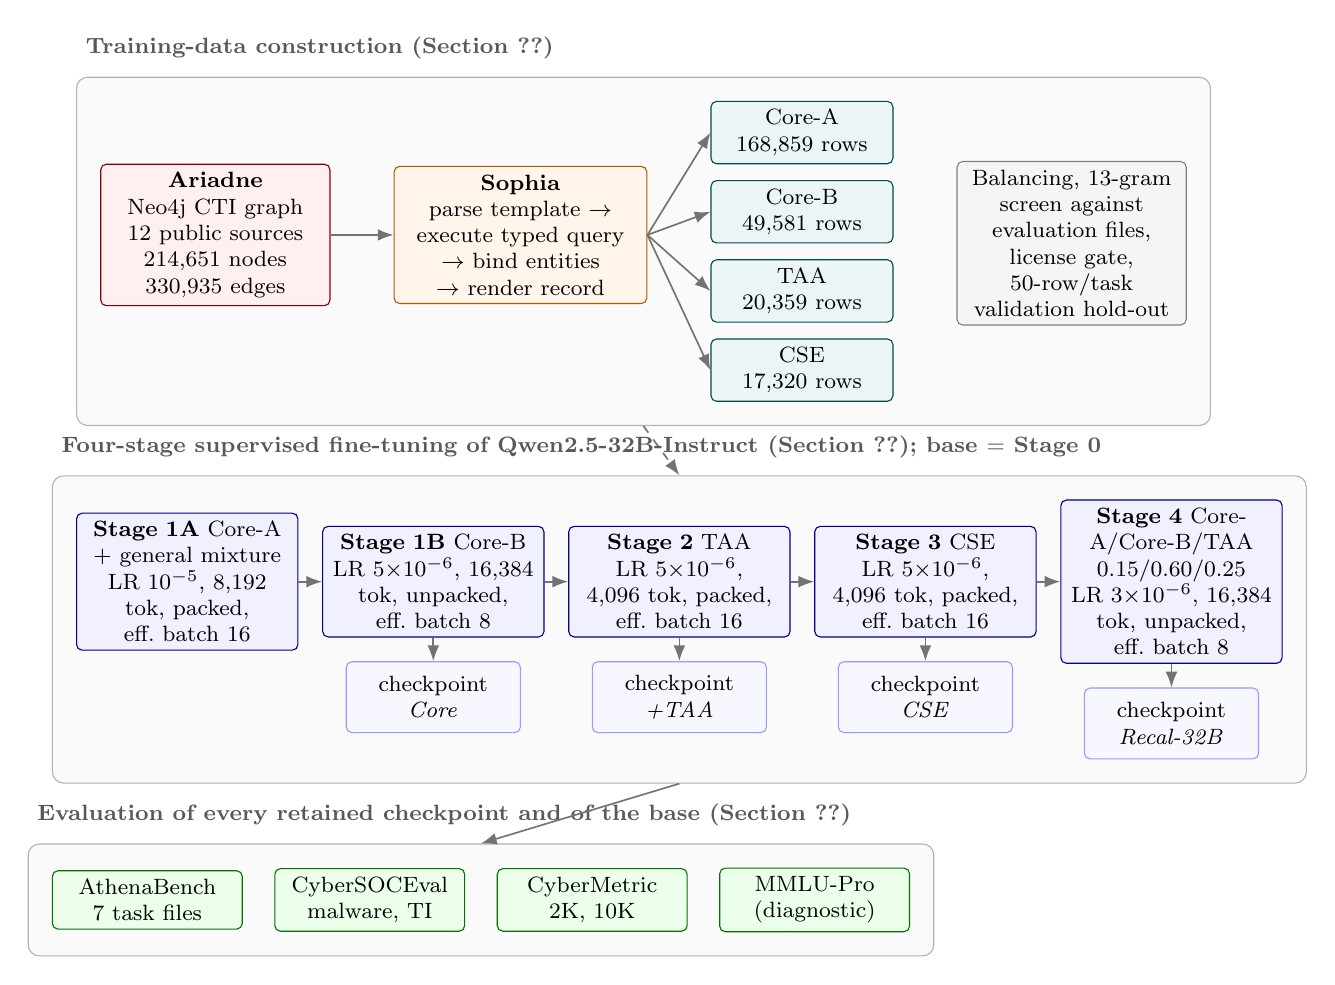
\begin{tikzpicture}[
  font=\footnotesize, >={Latex[length=2mm]}, node distance=3mm and 4mm,
  box/.style={draw, rounded corners=2pt, align=center, inner sep=3pt, minimum height=9mm},
  src/.style={box, fill=red!6, draw=red!55!black, text width=27mm},
  gen/.style={box, fill=orange!8, draw=orange!70!black, text width=30mm},
  shard/.style={box, fill=teal!8, draw=teal!60!black, text width=21mm, minimum height=7mm},
  stage/.style={box, fill=blue!6, draw=blue!55!black, text width=26mm},
  ev/.style={box, fill=green!8, draw=green!45!black, text width=22mm, minimum height=7mm},
  arr/.style={->, semithick, black!55}, grp/.style={draw=black!30, rounded corners=4pt, inner sep=3mm, fill=black!2},
  lbl/.style={font=\footnotesize\bfseries, text=black!65}]
\node[src] (ari) {\textbf{Ariadne}\\Neo4j CTI graph\\12 public sources\\214,651 nodes\\330,935 edges};
\node[gen, right=8mm of ari] (sop) {\textbf{Sophia}\\parse template $\to$ execute typed query $\to$ bind entities $\to$ render record};
\node[shard, right=8mm of sop, yshift=13mm] (sa) {Core-A\\168,859 rows};
\node[shard, below=2mm of sa] (sb) {Core-B\\49,581 rows};
\node[shard, below=2mm of sb] (st) {TAA\\20,359 rows};
\node[shard, below=2mm of st] (sc) {CSE\\17,320 rows};
\node[box, fill=black!4, draw=black!50, text width=27mm, right=8mm of sb, yshift=-4mm] (scr) {Balancing, 13-gram screen against evaluation files, license gate, 50-row/task validation hold-out};
\draw[arr] (ari) -- (sop);
\foreach \s in {sa,sb,st,sc} \draw[arr] (sop.east) -- (\s.west);
\begin{scope}[on background layer]
 \node[grp, fit=(ari)(sop)(sa)(sc)(scr)] (g1) {};
\end{scope}
\node[lbl, above=1mm of g1.north west, anchor=south west] {Training-data construction (Section~\ref{sec:data})};
% stages
\node[stage, below=11mm of g1.south west, anchor=north west] (s1) {\textbf{Stage 1A} Core-A + general mixture\\LR $10^{-5}$, 8,192 tok, packed, eff.\ batch 16};
\node[stage, right=3mm of s1] (s1b) {\textbf{Stage 1B} Core-B\\LR $5{\times}10^{-6}$, 16,384 tok, unpacked, eff.\ batch 8};
\node[stage, right=3mm of s1b] (s2) {\textbf{Stage 2} TAA\\LR $5{\times}10^{-6}$, 4,096 tok, packed, eff.\ batch 16};
\node[stage, right=3mm of s2] (s3) {\textbf{Stage 3} CSE\\LR $5{\times}10^{-6}$, 4,096 tok, packed, eff.\ batch 16};
\node[stage, right=3mm of s3] (s4) {\textbf{Stage 4} Core-A/Core-B/TAA 0.15/0.60/0.25\\LR $3{\times}10^{-6}$, 16,384 tok, unpacked, eff.\ batch 8};
\draw[arr] (s1) -- (s1b); \draw[arr] (s1b) -- (s2); \draw[arr] (s2) -- (s3); \draw[arr] (s3) -- (s4);
\node[box, fill=blue!3, draw=blue!40, text width=20mm, below=3mm of s1b] (c1) {checkpoint\\\emph{Core}};
\node[box, fill=blue!3, draw=blue!40, text width=20mm, below=3mm of s2] (c2) {checkpoint\\\emph{+TAA}};
\node[box, fill=blue!3, draw=blue!40, text width=20mm, below=3mm of s3] (c3) {checkpoint\\\emph{CSE}};
\node[box, fill=blue!3, draw=blue!40, text width=20mm, below=3mm of s4] (c4) {checkpoint\\\emph{Recal-32B}};
\draw[arr] (s1b) -- (c1); \draw[arr] (s2) -- (c2); \draw[arr] (s3) -- (c3); \draw[arr] (s4) -- (c4);
\begin{scope}[on background layer]
 \node[grp, fit=(s1)(s4)(c1)(c4)] (g2) {};
\end{scope}
\node[lbl, above=1mm of g2.north west, anchor=south west] {Four-stage supervised fine-tuning of Qwen2.5-32B-Instruct (Section~\ref{sec:training}); base $=$ Stage 0};
% eval
\node[ev, below=11mm of g2.south west, anchor=north west] (e1) {AthenaBench\\7 task files};
\node[ev, right=4mm of e1] (e2) {CyberSOCEval\\malware, TI};
\node[ev, right=4mm of e2] (e3) {CyberMetric\\2K, 10K};
\node[ev, right=4mm of e3] (e4) {MMLU-Pro\\(diagnostic)};
\begin{scope}[on background layer]
 \node[grp, fit=(e1)(e4)] (g3) {};
\end{scope}
\node[lbl, above=1mm of g3.north west, anchor=south west] {Evaluation of every retained checkpoint and of the base (Section~\ref{sec:evaluation})};
\draw[arr] (g2.south) -- (g3.north);
\draw[arr, dashed] (g1.south) -- (g2.north);
\end{tikzpicture}}
\caption{Glaukopis pipeline as configured for the reported v21 release. Shard sizes are the realized post-screen training rows; stage settings are read from the release launchers. The general mixture in Stage 1A (T\"ulu-3 SFT and Alpaca) is not Sophia-generated and is not screened against the evaluation files.}\label{fig:pipeline}
\end{figure*}

\begin{table*}
\centering\footnotesize
\caption{Pipeline boundaries. Provenance is strongest for Sophia-materialized CTI targets; it should not be generalized to all auxiliary data or to unconstrained model completions.}\label{tab:boundaries}
\begin{tabularx}{\textwidth}{@{}P{2.4cm}XXX@{}}
\toprule Component & Input and transformation & Resulting artifact & Scope of assurance \\\midrule
Ariadne & Public CTI records normalized to typed entities and relations & Neo4j CTI snapshot & Source-linked facts; not proof of source completeness or correctness \\
Sophia & Expert-authored template, typed query, graph binding, rendering & Instruction, context, and target record with template identifier & Target traceable to the executed graph binding \\
Corpus preparation & Generation, balancing, $n$-gram screening, license gate, phase splitting & Core-A, Core-B, TAA, CSE, and validation shards & Dependent on covered files, fields, thresholds, and retained reports \\
Supervised training & Stage-specific shard mixture and optimizer configuration & Core, +TAA, CSE, Recal-32B checkpoints & Observable transitions; no isolated scheduling effect \\
Evaluation & Fixed task inputs, checkpoint, parser and scorer, serving settings & Predictions, per-item scores, run manifests & Reproducible only to the extent the run manifests and artifacts are retained \\\bottomrule
\end{tabularx}
\end{table*}

\paragraph{How the sources were selected}
The twelve sources were chosen from a longer list of candidates surveyed when the project began (nineteen, including MISP galaxies, AlienVault OTX pulses, ThreatFox and other indicator feeds, Malpedia, APT Notes and vendor blogs, Project Zero and ZDI advisories, Rapid7 datasets, TRAM, BRON, and a commercial intelligence feed). Three criteria separate the selected sources from the rest, and each follows from the provenance goal. A source must publish machine-readable records with stable identifiers, so that a training target can name the record it came from; narrative sources such as blogs, advisories, and APT reports would have required a model to extract facts first, which breaks the chain from target to public record. A source must cross-reference other catalogs by identifier, so that it contributes edges and not only nodes; pure indicator feeds (addresses, hashes, domains) carry few such references and little of the reasoning the tasks require. And a source must permit redistribution of derived data under a license the build pipeline can check, which the corpus license gate enforces per row (Section~\ref{sec:corpus}) and which excludes commercial feeds. Sources that fail one of these criteria are not worse CTI; they are unsuitable as a substrate for traceable supervision.

\subsection{Sophia: template language, generation pipeline, and validation}\label{sec:sophia}
Sophia is the component that turns Ariadne into training data. A template is a short declarative document, authored by a CTI analyst, that fixes the role and task of an instruction, states a question in terms of graph entities, and states the answer in terms of the same entities and their relationships. Generation parses the template into a typed graph query, executes it against Ariadne, binds the returned entities and relationships, and renders one instruction record per binding (Figure~\ref{fig:pipeline}).

\paragraph{Template language}
A template binds graph nodes to local aliases, references their typed properties through dotted access, and emits the resolved values inside natural-language text. The simplest templates read one node:
\begin{lstlisting}
M.1 Instruction: You are a cybersecurity expert ... working in a SOC ...
Question: Explain ATT&CK technique {ap:attack-pattern.name} ({ap.id}) and how it is used.
Answer: Technique {ap.name} ({ap.id}) is described as follows: {ap.description}. It is commonly observed across {ap.x_mitre_platforms}.
\end{lstlisting}
Here \texttt{\{ap:attack-pattern.name\}} introduces \texttt{ap} as an alias for an ATT\&CK technique node and emits its name; later references reuse the binding. The language adds relationship traversal (written \texttt{\{a.rel>Type.prop\}}), equality and inequality constraints, any/all filters over list-valued properties, list expansion that renders every neighbor of a node, hidden sections that establish bindings or constraints without producing text, random selection among candidates, and a \texttt{source\#type} prefix that disambiguates labels shared across sources (an ATT\&CK attack pattern versus a CAPEC one). The following template correlates a CVE with its weakness and attack pattern across three catalogs:
\begin{lstlisting}
Question: Correlate CVE, CWE, and CAPEC for a single vulnerability chain.
Answer: CVE {cve:CVE.id} impacts CAPEC {cap:cve.impacts>CAPEC.name}
and is categorized as weakness {cwe:cve.problemType>Weakness.name}.
CAPEC {cap.id} exploits weakness {cwe2:cap.exploits>Weakness.name}.
<*{force cwe.id=cwe2.id}*>
\end{lstlisting}
The hidden equality constraint requires the two traversals (CVE to weakness directly, and CVE to attack pattern to weakness) to resolve to the same identifier, so that the rendered record states a fact the graph supports along both paths. A reviewer can inspect the binding rather than trust a separately synthesized answer. Negative constraints produce records that distinguish graph-supported from unsupported associations---a mitigation that does \emph{not} address a technique, a data component that does \emph{not} detect any technique a malware family uses---and are how the yes/no and negative-attribution families in the Core and TAA shards are generated. Absence of a relationship in an incomplete graph is not evidence that the relationship is false in the world, so negative records are interpreted against the declared graph under a documented closed-world assumption.

\paragraph{Record format and family identifiers}
Every generated record is a three-field Alpaca-format JSON object (\texttt{instruction}, \texttt{input}, \texttt{output}) carrying two additional fields: \texttt{shortname}, the identifier of the template that produced it (for example \texttt{AB.RCM.4} or \texttt{JS.CSE.TI.GRP.1}), and \texttt{source}. Template identifiers are hierarchical: the prefix names the family (\texttt{AB} for AthenaBench-schema drills, \texttt{JS} for JSON-answer drills, \texttt{SOC} for SOC triage and incident-response families, \texttt{YN} for yes/no, \texttt{X} and \texttt{CL} for cross-catalog and classification families, \texttt{V} and \texttt{POC} for vulnerability and proof-of-concept families), the middle element the task, and the suffix the variant. The shard profiles in Section~\ref{sec:cseshard} and the overlap audit in Section~\ref{sec:overlap} are computed over these identifiers, and Supplementary Material~S3 shows one verbatim record from each major family.

\paragraph{Generation pipeline}
A single wrapper script runs three steps. The first extracts templates from their authoring format (a Word document or a JSON file; analysts author in Word with inline \texttt{Instruction}, \texttt{Question}, and \texttt{Answer} markers) into a structured intermediate form. The second opens a connection to Ariadne, issues the query implied by each template, samples bindings up to a per-template ceiling, and writes one triple file per template together with a results report that records how many bindings each template produced and which templates failed to bind. The third merges the per-template files into one Alpaca-format shard. Two settings control shard size: the number of distinct bindings sampled per template and a cap on records per template; the row counts of the release are gated by a plan that sets a minimum number of rows for each task axis (ten axes for the Core shard), so that a family whose templates silently stop binding (for example after a source renames a property) fails the build rather than shrinking the corpus (Table~\ref{tab:gates}).

\paragraph{Balancing, screening, and validation hold-out}
After generation the shard is balanced across families, screened for verbatim overlap with the evaluation files (Section~\ref{sec:contamination}), checked against a per-row license allowlist, and split: 50 rows per template family are held out as a validation shard for loss monitoring during training, and the remainder is serialized as the training shard. Section~\ref{sec:corpus} gives the realized counts.

\paragraph{Schema validation}
Because templates reference graph labels, properties, and relationship types by name, a change in a source (a renamed property in a refreshed STIX bundle, a retired relationship type) can make a template bind nothing or bind the wrong thing. A separate schema-test module generates probe templates from the declared graph schema, runs them through the generation engine against the deployed graph, and reports every label, property, or relationship that a template references but the graph does not provide. This catches structural drift before it reaches training data. It does not catch semantic drift: a template whose query binds successfully to a record that is itself wrong or stale produces a record that is graph-consistent but incorrect, and the examples in Supplementary Material~S3 include two such cases. Graph-grounded generation guarantees that a target is traceable to its sources; it does not guarantee that the sources, or the template's reading of them, are right, and it does not guarantee graph-faithful answers from the trained model at inference time, which would require runtime retrieval or constrained decoding.

\paragraph{Quality checks and what they miss}
Table~\ref{tab:gates} collects the checks applied to the generated data, the class of defect each is designed to detect, and the class it cannot. Two of the build gates were added after a release failed silently. In release v11, four benchmark-aligned template families reached only 22--48\% of their planned row counts and one planned family produced no rows at all; the build completed, the model was trained, and the under-build was found only while diagnosing the release's benchmark regressions, which led to the row-count gate. In release v17, the parser that converts authored templates into the generator's input dropped the option lines from every multiple-select prompt, and the answer letters had been written into the templates instead of being shuffled with the options, so a single letter combination appeared in 50.7\% of the target rows and only four combinations occurred at all; the model learned to emit that combination regardless of input, and the release regressed on every AthenaBench task. The answer-letter balance gate added afterwards fails that corpus when it is run on it. No automated check caught the rendering defects reproduced in Supplementary Material~S3; they were found by reading sampled rows. The pattern is the familiar one from data validation for machine learning \citep{breck2019datavalidation}: cheap structural and distributional checks catch structural and distributional failures, and semantic correctness still requires a person reading samples of the data.

\begin{table*}
\centering\footnotesize
\caption{Quality checks applied to the generated data. All automated checks except the schema tests run as phases of each shard's build and halt it on failure; every check passed for the reported release, and the training launchers refuse to start without the shard files (Supplementary Material~S2).}\label{tab:gates}
\begin{tabularx}{\textwidth}{@{}P{4.2cm}XX@{}}
\toprule Check & What it detects & What it cannot detect \\\midrule
Graph substrate check (minimum node counts for seven entity classes and ten probe traversals, before generation) & An incomplete or mis-loaded graph & Wrong or stale records in a complete graph \\
Seed-provenance gate (registered provenance and SHA-256 hash for each external seed file of the auxiliary generators) & Unregistered or modified generator inputs & Errors in the registered content \\
Schema probe tests (run separately against the deployed graph) & Labels, properties, or relationship types that a template references but the graph lacks & Semantic drift: well-formed bindings to stale or wrong records \\
Row-count gate (minimum rows per task axis; ten axes for the Core shard) & Families that silently stop binding or under-produce & A family that produces enough rows of the wrong kind \\
Answer-letter balance gate (CSE shard) & Degenerate multiple-select targets: a letter that is almost never or almost always correct, a dominant letter combination, or too few distinct combinations & Wrong answers with a balanced letter distribution \\
Verbatim 13-gram screen against the evaluation files (Section~\ref{sec:contamination}) & Rows that reproduce indexed evaluation text (684 Core rows removed in the release) & Paraphrases; benchmarks absent from the index; the general mixture \\
Per-row license allowlist & Rows whose source tag is not on the redistribution allowlist & Errors in the license metadata itself \\
Validation hold-out (50 rows per family) & A family whose loss stops improving during training & Generalization beyond the template distribution \\
Sampled manual reading (not automated) & Rendering defects that are well-formed with respect to the graph (Supplementary Material~S3) & Anything outside the sample \\\bottomrule
\end{tabularx}
\end{table*}


\subsection{Corpus scope and reproducibility}\label{sec:corpus}
The reported v21 release uses four production CTI shards (Core-A, Core-B, TAA, and CSE) and three validation shards holding out 50 rows per template family. The build reports record the realized sizes: the Core corpus contained 219,675 rows after balancing, of which 684 were removed by the $n$-gram screen (Section~\ref{sec:contamination}), 550 were held out for validation, and of the remaining 218,441 training rows 168,859 were assigned to Core-A and 49,581 to Core-B (the phase-split report accounts for all but one row); the TAA and CSE shards contained 20,359 and 17,320 training rows. Core-A is trained together with a general-purpose instruction mixture (T\"ulu-3 SFT and Alpaca-English \citep{lambert2024tulu3,taori2023alpaca}), which is neither Sophia-generated nor screened. Consequently, the statement ``every training example is graph-materialized'' applies to Sophia-generated CTI records only.

The architecture ports use the same serialized CTI release. The release itself was built as a reproducibility experiment: its three template manifests, row-count gates, and per-template limits are byte-identical (hash-verified) to those of the preceding release, with only dataset names and output targets changed, and the sign-off criterion was that the post-Core checkpoint would land within 1.5 points of the predecessor's on every task. The aggregate did; two task scores (ATE and RCM) did not. Because the template inputs were identical, the most parsimonious explanation is non-determinism in the data build: exact row-level regeneration was not seed-pinned, since graph-read order, binding sampling, and deduplication tie-breaks can all vary between runs. Byte-identical templates therefore did not reproduce per-task scores within the intended tolerance, and the two intermediate releases between the predecessor and this one showed the same pattern. Template identity alone therefore does not certify identical training rows. A reproducible release needs hashes of the serialized files, per-source graph snapshots, counts after each filter, and software versions, in addition to the templates.

\section{Multi-stage training configuration}\label{sec:training}
\subsection{Base model and the rationale for the stages}
The base is \code{Qwen/Qwen2.5-32B-Instruct} \citep{qwen2025qwen25}, chosen for three reasons: it is openly licensed for local deployment; at 32B parameters it serves in bfloat16 on two 80-GB GPUs, which is the hardware a mid-sized SOC can allocate; and its zero-shot scores on CyberMetric (90.2) and MMLU-Pro (69.0) are high enough that losses of general capability are measurable against a strong baseline rather than hidden by a weak one. Additional ports to Qwen2.5-14B-Instruct, Qwen3-30B-A3B-Thinking-2507 \citep{yang2025qwen3}, Meta-Llama-3.1-8B-Instruct \citep{grattafiori2024llama3}, and Foundation-Sec-8B-Instruct \citep{kassianik2025foundationsec} test whether the recipe transfers across architecture and size; the mixture-of-experts (MoE) port has 30.5B total and 3.3B active parameters per token.

The four-stage schedule in Table~\ref{tab:training} was not designed a priori. It is the configuration the project converged on over twenty earlier releases on smaller bases, in which single mixed passes repeatedly improved some AthenaBench tasks while leaving the multiple-choice and attribution tasks near their base values (Section~\ref{sec:singlestage}). The schedule separates concerns in the order of increasing narrowness. Stage 1A trains the broad CTI families (knowledge questions, multiple choice, SOC triage, compliance, and yes/no families) together with a general instruction mixture, so that the model first sees the domain vocabulary without losing instruction-following behavior. Stage 1B trains the four catalog-mapping schemas (mitigation sets, technique extraction, severity vectors, root cause) at a longer context length because their prompts embed full CVE and technique descriptions. Stage 2 drills threat-actor attribution, whose answer space (ATT\&CK groups and their aliases) is small and had resisted improvement inside the broad mixture. Stage 3 drills the SOC-style multiple-select format used by CyberSOCEval, whose answers are letter sets. Stage 4 revisits a mixture of the Stage-1 and Stage-2 shards at a low learning rate to recover capabilities displaced by the two narrow drills. Each stage therefore has a stated purpose, and Section~\ref{sec:results} tests whether that purpose was achieved; retaining the checkpoint after each stage is what makes the test possible.

Training uses LlamaFactory \citep{zheng2024llamafactory} with DeepSpeed ZeRO-3 and CPU offload \citep{rajbhandari2020zero}, an 8-bit AdamW optimizer, Liger kernels, gradient checkpointing, and bfloat16 precision on eight 80-GB H100 GPUs; these are the standard choices for full-parameter fine-tuning of a 32B model on one node and were not varied. Effective batch size is preserved by adjusting gradient accumulation to the GPU count. Each stage runs for one epoch over its shard, so the number of updates per stage is determined by the shard size and the effective batch.

\begin{table*}
\centering\footnotesize
\caption{Canonical 32B training recipe read from the v21 launchers. Caps are the per-dataset \texttt{max\_samples} limits, not realized token counts. The general mixture is capped separately from Core-A because the limit applies per dataset. Wall-time budgets are the project's documented planning figures for eight H100 GPUs, not metered bills of the reported runs.}\label{tab:training}
\fitwidth{\begin{tabular}{@{}llrrrrll@{}}
\toprule Pass & Training input & Cap & Max.\ tokens & LR & Eff.\ batch & Packing & Budget (h) \\\midrule
1A & Core-A + T\"ulu-3 SFT + Alpaca & 240,000 & 8,192 & $1\times10^{-5}$ & 16 & on & \multirow{2}{*}{26--30} \\
1B & Core-B & 70,000 & 16,384 & $5\times10^{-6}$ & 8 & off & \\
2 & TAA & 33,000 & 4,096 & $5\times10^{-6}$ & 16 & on & 13--17 \\
3 & CSE & 33,000 & 4,096 & $5\times10^{-6}$ & 16 & on & 9--13 \\
4 & Core-A/Core-B/TAA at 0.15/0.60/0.25 & 3,600 per shard & 16,384 & $3\times10^{-6}$ & 8 & off & 3--4 \\\bottomrule
\end{tabular}}
\end{table*}

Because the caps exceed the realized Core-B, TAA, and CSE shard sizes, those passes consume their shards in one epoch. In pass 1A the cap applies to the Sophia shard and to each auxiliary dataset separately, so the general mixture can contribute up to 240,000 rows alongside the 168,859 Core-A rows; the auxiliary share is therefore material to the forgetting discussion in Section~\ref{sec:results}. Stage 4 interleaves the three shards under the stated probabilities up to the per-shard cap, which yields about 6,000 interleaved examples. Neither repeated exposure nor actual token consumption can be inferred from the caps; sequence limits are maxima, not average lengths.

The alternative Stage-4 recipe developed for the 14B port uses learning rate $10^{-6}$, mixture probabilities 0.25/0.40/0.35, and a 2,400-example cap. Both Stage-4 variants were trained from the same CSE parent on the 32B base and both are evaluated below. Applying different Stage-4 mixtures and rates across architectures means that the complete training treatment is not byte-identical across every port.

\subsection{What changes between stages}\label{sec:stagechanges}
Table~\ref{tab:training} makes explicit that four quantities change together at a stage boundary: the training data, the maximum sequence length, whether short examples are packed into one sequence, and the learning rate. This co-variation is deliberate from an engineering standpoint (each shard has its own natural context length, and the narrow drills use a lower rate than the broad pass), but it means that a difference between two consecutive checkpoints is the effect of the whole configuration change, not of the data alone. We call the retained models \emph{cumulative checkpoints}: they reveal the effect of continuing training under each configured treatment, and they are not matched ablations. A chain that skips the attribution stage was not trained, so the necessity of Stage 2 is not tested. The first retained checkpoint, however, is a single-stage model, and Section~\ref{sec:singlestage} uses it as the baseline against which the later stages are measured.

\subsection{The single-stage baseline}\label{sec:singlestage}
The four-stage design contains its own single-stage baseline. Stage 1 fine-tunes the base model once, on the Core shards, and its checkpoint is retained and evaluated with the same harness, prompts, and per-item records as every later checkpoint. The Core checkpoint is therefore the model that single-stage training on the release's core data produces, and Stages 2--4 are evaluated as increments over it: whatever they add or remove appears as a paired, item-level difference between a later checkpoint and Core (Table~\ref{tab:paired}, last column), which is a stronger comparison than one between separately trained models evaluated at different times. Stage 1 runs as two consecutive passes, a broad pass over Core-A with the general mixture and a longer-context pass over Core-B (Table~\ref{tab:training}), because the two shards need different sequence limits; it contains neither of the narrow drills nor the recalibration pass, which is the sense in which it is a single stage. Section~\ref{sec:fullchain} reports what the later stages contribute relative to it.

\paragraph{Earlier single-pass releases}
Before the staged design was adopted, the project trained single-pass models on earlier corpora. On the 32B base, one stage of three epochs over the release-v7 corpus (180,533 CTI rows at learning rate $10^{-5}$) reached 65.8 on the AthenaBench mean with Classic attribution only, against 66.5 for the released chain under the same convention. On the 14B development base, three single-pass releases reached 56.1 to 60.0 on that mean and the phased releases that followed reached 60.6 to 64.9. Each of these releases also changed the corpus, so they record why the project moved to stages; within the reported release, the contribution of the later stages is measured against the single-stage baseline.


\section{Evaluation protocol}\label{sec:evaluation}
\subsection{Task portfolio, scorers, and run records}
AthenaBench evaluates CTI knowledge (CKT), attack-technique extraction (ATE), root-cause mapping (RCM), risk-mitigation strategy (RMS), vulnerability-severity prediction (VSP), and threat-actor attribution (TAA) in Classic and Canonical forms \citep{alam2025athenabench}. CyberSOCEval supplies malware-analysis and threat-intelligence-reasoning tasks \citep{deason2025cybersoceval}; CyberMetric supplies cybersecurity multiple-choice evaluation at the 2K and 10K tiers \citep{tihanyi2024cybermetric}; MMLU-Pro is a general-task diagnostic \citep{wang2024mmlupro}. Table~\ref{tab:portfolio} lists the item counts and the scorer that the harness applies to each task, read from the evaluation code. Large language models were used in preparing this article only as writing and coding aids (editing the manuscript text, checking bibliographic records, and drafting the arithmetic-verification scripts that accompany it); no model generated any training row, evaluation item, result, or interpretation, and the authors verified every script and number. The scorers differ in kind, so task scores should not all be called accuracy or treated as calibrated probabilities of operational success.

\begin{table*}
\centering\footnotesize
\caption{Evaluation portfolio as executed for the 32B chain. Item counts are from the run manifests; scorer definitions are from the evaluation code. TAA and RMS ``combined'' scores award full credit for a strict match and half credit for a plausible match (an alias or related group for TAA; a mitigation from the technique's neighborhood for RMS).}\label{tab:portfolio}
\begin{tabularx}{\textwidth}{@{}lrX@{}}
\toprule Task & Items & Per-item score used in the aggregates \\\midrule
CKT (multiple choice) & 3,000 & 1 if the option letter matches \\
RCM & 2,000 & 1 if the CWE identifier matches exactly \\
VSP & 2,000 & $1-|s_{\text{pred}}-s_{\text{gold}}|/7.7$, with $s$ the CVSS v3.1 base score of the parsed vector \citep{first2019cvss}; unparseable vectors are excluded (two of 2,000 for the final checkpoint) \\
ATE & 500 & 1 if the technique matches at the parent-technique level (sub-technique suffix ignored) \\
RMS & 500 & Set F1 over predicted mitigation identifiers; combined variant credits neighborhood mitigations at half weight \\
TAA Classic & 100 & 1 alias-connected, 0.5 related group, 0 otherwise \\
TAA Canonical & 133 & 1 if the canonical group name or G-code appears, 0.5 if another alias of the group appears, 0 otherwise \\
CyberSOCEval malware / TI & 609 / 588 & Jaccard similarity between predicted and gold option-letter sets; strict accuracy is Jaccard $=1$; unparseable responses are excluded from both denominators \\
CyberMetric 2K / 10K & 2,000 / 10,180 & 1 if the option letter matches \\
MMLU-Pro & 12,032 & 1 if the extracted option letter matches (zero-shot chain-of-thought prompt) \\\bottomrule
\end{tabularx}
\end{table*}

Local checkpoints were served with vLLM \citep{kwon2023vllm} on two H100 GPUs at batch size 32 (64 for MMLU-Pro), and hosted references used the same harness through provider APIs \citep{glaukopis2026software}. The run manifests date the CTI evaluations of the five 32B checkpoints to 20--21 May 2026 and the MMLU-Pro evaluations to 23--26 May 2026. Each score is a single evaluation of a single training run. Item-level prediction and score files were retained for the five fine-tuned checkpoints and are the basis of the bootstrap and error analyses below; the corresponding files for the base model and the hosted references were not retained, so paired statistics involving them are not reported.

\subsection{Baselines and reference models}\label{sec:baselines}
Five kinds of comparison are reported, each controlling something different.
\begin{enumerate}
\item \emph{The base model}, Qwen2.5-32B-Instruct, evaluated zero-shot with the same prompts. Every fine-tuned score is read against it; this is the only comparison in which the architecture, parameter count, and serving configuration are held fixed.
\item \emph{A security-specialized open model}, Foundation-Sec-8B-Instruct \citep{kassianik2025foundationsec}, an 8B Llama-3.1 derivative continued-pretrained on cybersecurity text and instruction-tuned by its authors. It represents the alternative of adopting an existing domain model rather than specializing one, and it is also used as a base for one of the ports (Table~\ref{tab:ports}).
\item \emph{Six hosted frontier models}: GPT-5.5 and GPT-5.2 \citep{openai2026gpt55,openai2025gpt52}, DeepSeek-V4-Pro and DeepSeek-V3.2-Exp \citep{deepseek2026v4,deepseek2025v32exp}, and Gemini-3-Flash-Preview and Gemini-2.5-Flash \citep{google2025gemini3flash,comanici2025gemini25}, evaluated through provider APIs with the same harness and prompts (Table~\ref{tab:frontier}). They bound what is achievable without local deployment and without specialization.
\item \emph{The single-stage baseline}: the Core checkpoint, which Stage 1 produces by fine-tuning the base once on the core shards (Section~\ref{sec:singlestage}). It shares the base, harness, and per-item records with every later checkpoint, so the contribution of the later stages is measured by paired differences against it.
\item \emph{Four architecture ports} of the same recipe (Table~\ref{tab:ports}), which test transfer across model families and sizes.
\end{enumerate}
No comparison with other published CTI fine-tuning systems is made at the level of scores: CyberPal.AI and SecKnowledge \citep{levi2025cyberpal} and the systems in Table~\ref{tab:positioning} do not release weights evaluated on this suite, so a score comparison would require retraining them under our protocol, which was outside the project's budget. Their comparison in Table~\ref{tab:positioning} is therefore architectural, and we say so.

\subsection{Evaluation independence}\label{sec:independence}
The three CTI benchmarks differ in their independence from the training data. AthenaBench is aligned by design: Core-B trains the schemas assessed by its mapping and mitigation tasks, Stage 2 targets its attribution task, and Core-A includes multiple-choice families of the kind its knowledge task uses. It was also built by a team that includes one of the present authors. CyberSOCEval was built by Meta and CrowdStrike and CyberMetric by an unrelated academic group; neither was consulted when the templates were written, although Stage 3 does target CyberSOCEval's multiple-select answer format. MMLU-Pro is unrelated to the domain. The results are therefore reported in three tiers: AthenaBench measures whether the model learned the schemas it was trained on; CyberSOCEval and CyberMetric measure whether that learning transfers to CTI questions written by others; and MMLU-Pro measures what the specialization cost. Section~\ref{sec:overlap} quantifies, for AthenaBench, how often a test item's entities and gold answer occur in a training row, and reports scores on the items where they do not. Sharing public catalogs is appropriate for measuring public-catalog competence, but it does not establish generalization to unseen facts, new incidents, or private SOC telemetry, and an entity-disjoint or temporally held-out incident set remains the test that would.

\subsection{Contamination screening: what was run and what it covered}\label{sec:contamination}
Before training, each shard was scanned for verbatim overlap with the evaluation files. The filter lowercases alphanumeric word tokens and indexes distinct 13-word sequences; a single shared sequence flags a row for audit, and at least 50 shared sequences with one indexed evaluation record trigger removal. Table~\ref{tab:ngram} reports the retained build reports. The Core corpus had 34,897 flagged rows (15.9\%), almost all against the AthenaBench RCM, ATE, RMS, and VSP files, and 684 rows (0.3\%) were removed, chiefly VSP and RCM template rows that reproduced CVE descriptions at length. The TAA shard had no flagged row; the CSE shard had 41 flagged rows and none removed. Flagged-but-retained rows share between one and 49 thirteen-grams with an evaluation record; for a record of $L$ tokens the number of distinct 13-grams is at most $L-12$, so a complete duplicate of an evaluation record shorter than 62 tokens can never reach the removal threshold. The retained-overlap band is therefore a documented property of the method, not evidence that a particular test item was memorized.

\begin{table*}
\centering\footnotesize
\caption{Verbatim 13-gram screen as executed in the v21 build (build reports, May 2026). ``Flagged'' rows share at least one 13-gram with an indexed evaluation record and are shown by their maximum number of shared 13-grams with a single record; rows at 50 or more were removed. The index held 808,440 distinct 13-grams from 18 files.}\label{tab:ngram}
\fitwidth{\begin{tabular}{@{}lrrrrrrrrr@{}}
\toprule & & \multicolumn{6}{c}{Flagged rows by maximum shared 13-grams} & & \\\cmidrule(lr){3-8}
Shard & Scanned & 1 & 2--4 & 5--12 & 13--24 & 25--49 & $\ge$50 (removed) & Flagged total & Retained \\\midrule
Core & 219,675 & 6,641 & 10,952 & 6,656 & 3,165 & 6,799 & 684 & 34,897 (15.9\%) & 218,991 \\
TAA & 20,509 & 0 & 0 & 0 & 0 & 0 & 0 & 0 & 20,509 \\
CSE & 17,670 & 24 & 17 & 0 & 0 & 0 & 0 & 41 (0.2\%) & 17,670 \\\bottomrule
\end{tabular}}
\end{table*}

Coverage is narrower than the project documentation implies. The 18 indexed files were the AthenaBench task files, the CyberMetric files, and two operational CVE and URL feeds. The CyberSOCEval question files are fetched into the evaluation directory at run time and were not present when the shards were built, so the CSE shard was screened only against AthenaBench and CyberMetric; the CTIBench tab-separated files were also outside the JSON glob. The auxiliary T\"ulu-3 and Alpaca mixtures were not screened at all, and base-model pretraining contamination is outside scope. Index keys use the file basename and row index, and only selected text fields are extracted. Hash-based exact deduplication, full-path identifiers, and a CyberSOCEval scan should be added before ``decontaminated'' is used without qualification.

\subsection{Entity and gold-fact overlap}\label{sec:overlap}
Verbatim screening cannot detect the case that matters most for a graph-generated corpus: a training row that states the evaluated fact in different words. We therefore measured, for each AthenaBench task, whether the evaluation item's entities and its gold answer co-occur in a single training row (Table~\ref{tab:overlap}). Technique identifiers are a bounded catalog and every ATE and RMS target appears in training, as expected for catalog competence. Of the 2,000 RCM items, 660 CVE identifiers appear somewhere in the Core shard and 137 items (6.9\%) have their exact CVE-to-CWE gold pair stated in one row. For VSP, 446 CVE identifiers appear but only seven items have their exact CVSS vector co-located with the identifier. For RMS, 273 of 500 items (54.6\%) have the technique's full gold mitigation set listed in one row, because catalog-listing templates enumerate a technique's mitigations. For Canonical TAA, 38 of 133 alias-to-group pairs are stated in a Core row.

\begin{table*}
\centering\footnotesize
\caption{Overlap between the v21 training shards and AthenaBench items, and the final checkpoint's mean item score on overlapping versus non-overlapping items. ``Gold fact in one row'' means that the item's identifying entity and its complete gold answer co-occur in a single training row of the Core shard (Core, TAA, and CSE shards for Canonical TAA). Scores are the per-item metrics of Table~\ref{tab:portfolio}.}\label{tab:overlap}
\fitwidth{\begin{tabular}{@{}lrrrrr@{}}
\toprule Task & Items & Entity in training & Gold fact in one row & Recal-32B: fact in training & Recal-32B: fact absent \\\midrule
RCM & 2,000 & 660 (33.0\%) & 137 (6.9\%) & 66.4 ($n{=}137$) & 64.3 ($n{=}1{,}340$)$^{a}$ \\
VSP & 2,000 & 446 (22.3\%) & 7 (0.4\%) & 77.4 ($n{=}445$)$^{b}$ & 77.9 ($n{=}1{,}553$) \\
ATE & 500 & 500 (100\%) & n/a & 70.5 (top tertile)$^{c}$ & 62.3 (bottom tertile) \\
RMS & 500 & 500 (100\%) & 273 (54.6\%) & 53.8 ($n{=}273$) & 73.1 ($n{=}227$) \\
TAA Canonical & 133 & 40 aliases (30.1\%) & 38 (28.6\%) & 7.9 ($n{=}38$) & 1.6 ($n{=}93$) \\\bottomrule
\end{tabular}}\par\smallskip
{\scriptsize $^{a}$Items whose CVE appears without the gold pair score 74.2 ($n{=}523$). $^{b}$CVE present in training (any row) versus absent. $^{c}$Items grouped by how often the gold technique occurs in training rows (tertile cuts at 156 and 298 rows; middle tertile 64.7).\par}
\end{table*}

The subset scores do not show the pattern expected from memorization of leaked facts. RCM items whose gold pair appears in training score within about two points of items whose CVE never appears; RMS items whose full mitigation set appears in training score lower, because those are the techniques with large mitigation sets on which set-F1 is hardest; VSP is unchanged. Two tasks do track exposure: ATE accuracy rises with the training frequency of the gold technique, and at the +TAA checkpoint Canonical-TAA items whose alias-to-group mapping appears in training score 52.6 against 30.6 for the remainder. These are the expected signatures of catalog competence rather than of test-item leakage, and they identify attribution as the task most dependent on explicit fact exposure. Semantic paraphrases of evaluation narratives, reused public facts, and benchmark-guided recipe selection remain uncontrolled; an entity-disjoint or temporally held-out incident set is still required for an out-of-sample claim.

\subsection{Explicit aggregation and the corrected attribution convention}\label{sec:aggregation}
To avoid hiding the Canonical-TAA regression, we define a balanced attribution score, an AthenaBench macro-score, and a three-benchmark mean:
\begin{align}
 \Tbal &= \tfrac12\,(T_{\mathrm{Classic}}+T_{\mathrm{Canonical}}),\\
 \Abal &= \tfrac16\,(K+E+R+M+V+\Tbal),\\
 \Bbal &= \tfrac13\,(\Abal+C+Y).
\end{align}
Here $K,E,R,M,V$ denote CKT, ATE, RCM, combined RMS, and VSP; $Y$ is the mean of the two CyberMetric tiers; and $C$ is the CyberSOCEval composite used throughout the project's results workbook for every row, including the hosted references, namely the mean of malware strict accuracy, malware Jaccard score, and threat-intelligence strict accuracy. That composite omits the threat-intelligence Jaccard score; a symmetric four-metric mean would change $\Bbal$ by at most 2.7 points for the rows reported here and would not change the base-to-final gain by more than 0.2 points. We retain the project convention so that every row is computed identically and state it explicitly.

Two further aggregates appear in the tables. The \emph{ten-test mean} averages CKT, ATE, RCM, strict RMS F1, VSP, $\Tbal$, the two strict CyberSOCEval accuracies, and the two CyberMetric tiers with equal weight; it is the project's long-standing leaderboard number and is reported for continuity. MMLU-Pro is never averaged into a CTI score, because a general-task diagnostic and a domain score measure different things. Earlier project documents report a composite in which the fine-tuned and base rows used Classic attribution alone while the hosted rows used $\Tbal$ (66.3 for the final checkpoint, 59.0 for the base); under the uniform $\Tbal$ convention those values are 65.0 and 57.7, and the gain is unchanged at 7.3 points. Every number in this article was recomputed from the per-item artifacts and run manifests under the conventions stated here.

\subsection{Uncertainty}\label{sec:uncertainty}
For the five fine-tuned checkpoints we computed 95\% percentile bootstrap intervals by resampling evaluation items with replacement (2,000 replicates), independently within each task and jointly for the aggregates \citep{efron1993bootstrap}. Differences between checkpoints use the same resampled items for both members of a pair, so they are paired estimates. These intervals quantify item-sampling uncertainty for a fixed trained model only. They say nothing about the variance of training itself, which would require independently seeded runs of the same recipe, and clustered items (for example, several CyberSOCEval questions drawn from one report) are treated as independent, which makes the intervals slightly optimistic for that benchmark.

\section{Results: adaptation, interference, and transfer}\label{sec:results}
\subsection{The canonical 32B chain}
Table~\ref{tab:stage} reports the task scores of the base model and the five retained checkpoints together with the aggregates of Section~\ref{sec:aggregation}; the ten-test means of the chain are 61.6, 61.7, 62.4, 62.4, and 62.9 against 49.6 for the base. Relative to the base, the final checkpoint improves ATE by 47.6 points, RMS by 54.9, CKT by 22.6, and RCM by 7.6; VSP decreases by 1.0 point, and MMLU-Pro by 11.6. The balanced AthenaBench score rises from 40.3 to 62.6 and the three-benchmark mean from 57.7 to 65.0. The item-bootstrap interval for the final checkpoint's $\Bbal$ is 64.1--66.0 and for $\Abal$ is 61.5--63.7; no paired interval with the base is available, but an unpaired normal approximation from the base's reported accuracies and item counts gives half-widths below 2.5 points for every accuracy task except ATE (3.4), so the base-to-final gain is far outside item-sampling noise.

\begin{table*}
\centering\scriptsize
\setlength{\tabcolsep}{3.3pt}
\caption{Task scores and aggregates for the canonical Qwen2.5-32B chain (single evaluation per checkpoint; 0--100 scale). $\Abal$ and $\Bbal$ follow Section~\ref{sec:aggregation} and are computed from the displayed rounded task scores; recomputing them from unrounded item scores changes them by at most 0.1. Recal-14B is the alternative Stage-4 recipe trained from the same CSE parent. The last row gives the half-width (larger side) of the final checkpoint's 95\% item-bootstrap interval.}\label{tab:stage}
\setlength{\tabcolsep}{2.8pt}
\fitwidth{\begin{tabular}{@{}lrrrrrrrrrrrr@{}}
\toprule Checkpoint & CKT & ATE & RCM & RMS & VSP & TAA Cl. & TAA Can. & $C$ & $Y$ & MMLU-Pro & $\Abal$ & $\Bbal$ \\\midrule
Base & 52.9 & 18.2 & 59.5 & 7.6 & 78.8 & 48.0 & 2.0 & 42.6 & 90.2 & 69.0 & 40.3 & 57.7 \\
Core & 72.9 & 67.2 & 69.8 & 63.8 & 83.1 & 46.5 & 18.4 & 31.1 & 89.6 & 59.2 & 64.9 & 61.9 \\
+TAA & 75.4 & 63.4 & 69.0 & 62.9 & 83.5 & 47.0 & 36.8 & 29.8 & 89.4 & 58.2 & 66.0 & 61.7 \\
CSE & 72.5 & 63.4 & 67.7 & 63.7 & 78.9 & 53.5 & 3.4 & 42.0 & 88.8 & 54.2 & 62.4 & 64.4 \\
Recal-14B & 76.0 & 61.6 & 68.3 & 63.6 & 75.7 & 50.5 & 5.6 & 42.4 & 89.2 & 54.6 & 62.2 & 64.6 \\
Recal-32B & 75.5 & 65.8 & 67.1 & 62.5 & 77.8 & 50.5 & 3.4 & 42.6 & 89.8 & 57.4 & 62.6 & 65.0 \\
\multicolumn{1}{@{}r}{\scriptsize 95\% half-width} & $\pm$1.6 & $\pm$4.4 & $\pm$2.0 & $\pm$3.4 & $\pm$1.1 & $\pm$5.5 & $\pm$3.0 & $\pm$2.5 & $\pm$0.7 & $\pm$1.0 & $\pm$1.1 & $\pm$1.0 \\
\bottomrule
\end{tabular}}
\end{table*}

The cross-benchmark gain is not spread across the three benchmark families. The AthenaBench term contributes $+7.4$ to the 7.3-point change in $\Bbal$, the CyberSOCEval term contributes zero (42.6 to 42.6), and the CyberMetric term contributes $-0.1$. The entire positive contribution therefore comes from the benchmark that the training shards target most directly. This is useful evidence of schema adaptation, not evidence of uniform gains across independently targeted CTI workloads.

Why the two external benchmarks do not move is explained by what they measure. CyberMetric is a knowledge test on which the base model already scores 90.2; the training data adds catalog facts the base largely knows, and the fine-tuned checkpoints neither gain nor lose more than a point, which is the expected result of specialization that does not damage general security knowledge. CyberSOCEval's composite is flat for a different reason: its two components move in opposite directions across the chain (Figure~\ref{fig:trajectories}). Malware-analysis accuracy falls from 24.1 to 7.8 after Stage 1, when the model has learned to answer with a single technique or identifier and no longer produces the multi-select letter set the task requires, and recovers to 26.4 only after Stage 3 teaches that format; threat-intelligence accuracy follows the same path (49.9 to 41.1 to 48.9) without quite regaining the base. The final composite therefore reflects a format recovered rather than reasoning gained, and the benchmark should not be read as showing transfer of CTI knowledge from the training data. The improvement on AthenaBench is itself concentrated in the tasks whose answer is a catalog identifier chosen from a bounded space (RMS, ATE, CKT), which is where a model that has been shown the catalog in the right format gains most and where a benchmark-aligned corpus is most likely to help; RCM, whose answer requires judging a free-text description, improves by 7.6 points, and VSP, which requires judging eight metrics, does not improve at all.

\subsection{What each transition reveals}
Figure~\ref{fig:trajectories} and Table~\ref{tab:paired} show the transitions with their paired intervals. The attribution stage raises Canonical TAA from 18.4 to 36.8 ($+18.4$, interval $+12.4$ to $+24.4$) and CKT by 2.6 points, with no reliable change elsewhere; under the balanced aggregation, AthenaBench peaks at this checkpoint (66.0), not at the released one.

\begin{figure*}
\centering
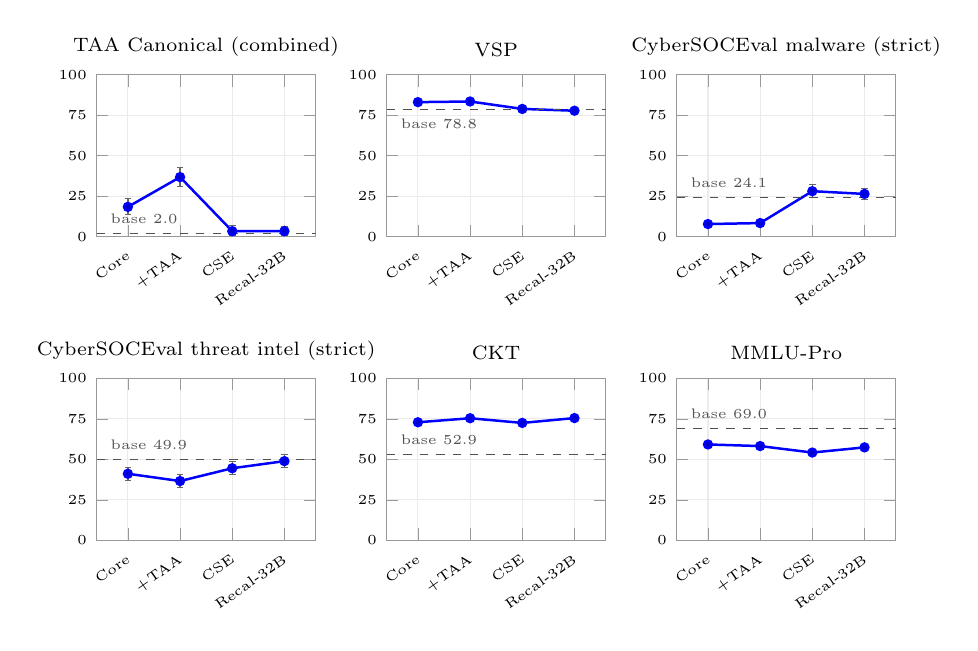
\begin{tikzpicture}
\begin{groupplot}[
  %% vertical sep must clear the rotated x tick labels of the upper row; at 13mm
  %% the lower row's titles printed on top of them.
  group style={group size=3 by 2, horizontal sep=9mm, vertical sep=18mm},
  width=0.36\textwidth, height=0.3\textwidth,
  ymin=0, ymax=100, ytick={0,25,50,75,100},
  xmin=-0.6, xmax=3.6, xtick={0,1,2,3}, xticklabels={Core,+TAA,CSE,Recal-32B}, x tick label style={font=\tiny, rotate=35, anchor=north east},
  y tick label style={font=\tiny}, title style={font=\scriptsize, yshift=-1mm},
  axis line style={black!40}, tick style={black!40}, grid=major, grid style={black!8},
  every axis plot/.append style={seriesblue, mark=*, mark size=1.4pt, line width=0.9pt, error bars/y dir=both, error bars/y explicit, error bars/error bar style={black!60, line width=0.5pt}, error bars/error mark options={black!60, rotate=90, mark size=1.2pt}}]
\nextgroupplot[title={TAA Canonical (combined)}]
\addplot coordinates {(0,18.4)+=(0,5.3)-=(0,4.9) (1,36.8)+=(0,5.7)-=(0,5.6) (2,3.4)+=(0,3.4)-=(0,2.6) (3,3.4)+=(0,3.0)-=(0,2.6)};
\draw[refgray, dashed] (axis cs:-0.6,2.0) -- (axis cs:3.6,2.0) node[pos=0.02, above right, font=\tiny, text=refgray] {base 2.0};
\nextgroupplot[title={VSP}]
\addplot coordinates {(0,83.1)+=(0,0.7)-=(0,0.7) (1,83.5)+=(0,0.6)-=(0,0.7) (2,78.9)+=(0,1.0)-=(0,1.0) (3,77.8)+=(0,1.1)-=(0,1.1)};
\draw[refgray, dashed] (axis cs:-0.6,78.8) -- (axis cs:3.6,78.8) node[pos=0.02, below right, font=\tiny, text=refgray] {base 78.8};
\nextgroupplot[title={CyberSOCEval malware (strict)}]
\addplot coordinates {(0,7.8)+=(0,2.3)-=(0,2.2) (1,8.4)+=(0,2.4)-=(0,2.2) (2,28.1)+=(0,4.1)-=(0,4.0) (3,26.4)+=(0,3.6)-=(0,3.5)};
\draw[refgray, dashed] (axis cs:-0.6,24.1) -- (axis cs:3.6,24.1) node[pos=0.02, above right, font=\tiny, text=refgray] {base 24.1};
\nextgroupplot[title={CyberSOCEval threat intel (strict)}]
\addplot coordinates {(0,41.1)+=(0,3.9)-=(0,4.0) (1,36.6)+=(0,3.8)-=(0,3.9) (2,44.5)+=(0,4.2)-=(0,4.1) (3,48.9)+=(0,4.1)-=(0,4.2)};
\draw[refgray, dashed] (axis cs:-0.6,49.9) -- (axis cs:3.6,49.9) node[pos=0.02, above right, font=\tiny, text=refgray] {base 49.9};
\nextgroupplot[title={CKT}]
\addplot coordinates {(0,72.9)+=(0,1.5)-=(0,1.6) (1,75.4)+=(0,1.6)-=(0,1.6) (2,72.5)+=(0,1.6)-=(0,1.6) (3,75.5)+=(0,1.6)-=(0,1.5)};
\draw[refgray, dashed] (axis cs:-0.6,52.9) -- (axis cs:3.6,52.9) node[pos=0.02, above right, font=\tiny, text=refgray] {base 52.9};
\nextgroupplot[title={MMLU-Pro}]
\addplot coordinates {(0,59.2)+=(0,0.9)-=(0,0.8) (1,58.2)+=(0,0.9)-=(0,0.9) (2,54.2)+=(0,0.9)-=(0,0.9) (3,57.4)+=(0,1.0)-=(0,0.9)};
\draw[refgray, dashed] (axis cs:-0.6,69.0) -- (axis cs:3.6,69.0) node[pos=0.02, above right, font=\tiny, text=refgray] {base 69.0};
\end{groupplot}
\end{tikzpicture}
\caption{Six task scores across the retained checkpoints of the canonical chain (points) with 95\% item-bootstrap intervals (bars) and the base model's score as a dashed reference. Intervals for the base are not available. The panels share one 0--100 axis; Stage 3 (CSE) raises the SOC-style tasks and collapses canonical attribution and part of VSP, and Stage 4 recovers CKT and MMLU-Pro but neither attribution nor VSP.}\label{fig:trajectories}
\end{figure*}

\begin{table*}
\centering\scriptsize
\setlength{\tabcolsep}{3.5pt}
\caption{Paired differences between checkpoints (later minus earlier) with 95\% paired item-bootstrap intervals; intervals that exclude zero are marked with an asterisk. These quantify item-sampling uncertainty for the specific trained models, not training-seed variance.}\label{tab:paired}
\fitwidth{\begin{tabular}{@{}lrrrr@{}}
\toprule Metric & +TAA $-$ Core & CSE $-$ +TAA & Recal-32B $-$ CSE & Recal-32B $-$ Core \\\midrule
CKT & $+2.6$ \ci{+1.0}{+4.2}* & $-3.0$ \ci{-4.5}{-1.4}* & $+3.1$ \ci{+1.5}{+4.6}* & $+2.7$ \ci{+1.1}{+4.2}* \\
ATE & $-3.8$ \ci{-7.6}{+0.2} & $0.0$ \ci{-4.8}{+4.6} & $+2.4$ \ci{-2.4}{+7.2} & $-1.4$ \ci{-5.2}{+2.8} \\
RCM & $-0.8$ \ci{-1.3}{-0.2}* & $-1.3$ \ci{-2.2}{-0.4}* & $-0.6$ \ci{-1.9}{+0.8} & $-2.7$ \ci{-3.9}{-1.5}* \\
RMS & $-1.0$ \ci{-3.3}{+1.6} & $+0.9$ \ci{-1.5}{+3.3} & $-1.2$ \ci{-3.9}{+1.5} & $-1.3$ \ci{-4.0}{+1.4} \\
VSP & $+0.3$ \ci{-0.1}{+0.7} & $-4.5$ \ci{-5.5}{-3.5}* & $-1.1$ \ci{-2.3}{0.0} & $-5.3$ \ci{-6.4}{-4.2}* \\
TAA Classic & $+0.5$ \ci{-5.0}{+6.0} & $+6.5$ \ci{+1.0}{+12.5}* & $-3.0$ \ci{-8.5}{+2.5} & $+4.0$ \ci{-1.5}{+9.5} \\
TAA Canonical & $+18.4$ \ci{+12.4}{+24.4}* & $-33.5$ \ci{-39.8}{-27.1}* & $0.0$ \ci{-3.0}{+2.6} & $-15.0$ \ci{-20.7}{-9.4}* \\
CSE malware (strict) & $+0.6$ \ci{-0.4}{+1.6} & $+19.7$ \ci{+15.3}{+24.2}* & $-1.8$ \ci{-4.5}{+1.0} & $+18.6$ \ci{+14.9}{+22.5}* \\
CSE threat intel (strict) & $-4.5$ \ci{-6.7}{-2.3}* & $+7.9$ \ci{+3.3}{+12.4}* & $+4.4$ \ci{+1.8}{+7.2}* & $+7.9$ \ci{+3.6}{+12.0}* \\
CyberMetric 10K & $-0.3$ \ci{-0.6}{0.0} & $-0.3$ \ci{-0.7}{+0.1} & $+0.8$ \ci{+0.5}{+1.2}* & $+0.2$ \ci{-0.2}{+0.6} \\
MMLU-Pro & $-1.0$ \ci{-1.7}{-0.4}* & $-4.0$ \ci{-4.8}{-3.2}* & $+3.2$ \ci{+2.5}{+3.9}* & $-1.8$ \ci{-2.6}{-1.1}* \\
$\Abal$ & $+1.1$ \ci{+0.1}{+2.2}* & $-3.6$ \ci{-4.8}{-2.3}* & $+0.2$ \ci{-0.9}{+1.3} & $-2.3$ \ci{-3.4}{-1.1}* \\
$\Bbal$ & $-0.1$ \ci{-0.6}{+0.4} & $+2.7$ \ci{+1.7}{+3.8}* & $+0.6$ \ci{-0.2}{+1.4} & $+3.2$ \ci{+2.2}{+4.2}* \\
\bottomrule
\end{tabular}}
\end{table*}

The Core transition produces the largest changes in the chain because it is the only stage that teaches the four mapping schemas: RMS rises from 7.6 to 63.8 and ATE from 18.2 to 67.2 chiefly because the base model, asked for mitigation identifiers or a technique code, produces prose or the wrong identifier family, whereas after Core-B it produces the requested identifiers in the requested final-line format. The gain is therefore partly format compliance and partly catalog recall, and the record does not separate the two. The attribution stage behaves as intended: it is the only transition that moves Canonical TAA upward, and Table~\ref{tab:taataxonomy} shows how, by converting ``wrong but known group'' answers (78 to 32) into correct-group answers under an alias (31 to 64) and exact answers (9 to 17). The model learns which group the tradecraft belongs to before it learns the group's canonical name.

Stage 3 raises CyberSOCEval malware strict accuracy by 19.7 points and threat-intelligence accuracy by 7.9 relative to +TAA, but Canonical TAA falls by 33.5 points (interval $-39.8$ to $-27.1$), VSP by 4.5, CKT by 3.0, and MMLU-Pro by 4.0, all outside their intervals. Classic TAA rises by 6.5. Stage 3 also introduces parsing failures: 17.1\% of malware responses could not be parsed at the CSE checkpoint against 0.7\% at Core, and because the scorer excludes unparseable responses, the malware accuracy with failures counted as wrong is 23.3 rather than 28.1. Section~\ref{sec:cseshard} shows that these effects follow from the content of the CSE shard. The recovery stage does not meet its objective of restoring VSP: 77.8 is below both its CSE parent (78.9) and the base (78.8), and Canonical TAA stays at 3.4. It does recover CKT ($+3.1$), MMLU-Pro ($+3.2$), threat-intelligence accuracy ($+4.4$), and both CyberMetric tiers, and it lowers the malware parsing-failure rate to 5.9\%. The resulting $\Bbal$ increase of 0.6 has an interval that includes zero. That Stage 4 recovers the broad capabilities but not the two narrow ones is consistent with its composition: at the 3,600-row cap and 0.25 mixture weight it re-exposes the model to about 900 attribution rows and 3,600 Core-B rows at a learning rate of $3\times10^{-6}$, against 17,320 rows of the competing format at $5\times10^{-6}$ in the stage before. A recalibration pass that is a fraction of the size of the pass it is correcting can restore behaviors that were only weakened (multiple-choice answering, general reasoning) but not behaviors that were replaced (G-code emission, exploitability judgments).

The label ``ship'' in the project denotes the released checkpoint, not a statistically established optimum. Relative to the CSE parent, the 14B-derived recipe loses 3.3 VSP points (interval $-4.4$ to $-2.2$) where the 32B-specific recipe loses 1.1; in a direct paired comparison the 32B-specific recipe is better on VSP ($+2.2$, interval $+1.0$ to $+3.4$), ATE ($+4.2$, $+0.2$ to $+8.2$), and MMLU-Pro ($+2.8$, $+2.1$ to $+3.4$), and worse on nothing beyond noise; the aggregate difference of 0.4 $\Bbal$ points has an interval that includes zero. Both are single training runs, so repeated seeds under a frozen selection rule are still needed to distinguish a robust recipe effect from training stochasticity.

\subsection{The full chain against the single-stage baseline}\label{sec:fullchain}
Taken together, the three stages after the single-stage baseline raise the three-benchmark mean by 3.2 points (paired interval $+2.2$ to $+4.2$; Table~\ref{tab:paired}, last column), from 61.9 at Core to 65.0. Of the released checkpoint's 7.3-point gain over the base model, about 4 points are therefore delivered by the single stage and about 3 by the later stages. Their contribution is concentrated on CyberSOCEval, where strict accuracy rises by 18.6 points on malware analysis and 7.9 on threat intelligence, and on CTI knowledge ($+2.7$). It is paid for on the aligned benchmark, where the balanced AthenaBench score falls by 2.3 points, Canonical attribution by 15.0, severity prediction by 5.3, and root-cause mapping by 2.7, and on MMLU-Pro ($-1.8$); every one of these intervals excludes zero. The staged schedule thus buys a net gain on the cross-benchmark mean by trading aligned-benchmark capability for SOC-format competence, and most of the trade happens at Stage 3 (Section~\ref{sec:cseshard}). A deployment that needs severity judgments or canonical attribution is better served by the single-stage checkpoint, and one that needs SOC-style multiple-select answers by the full chain; retaining both checkpoints is what makes that choice available.

\subsection{Why canonical attribution collapses}\label{sec:cseshard}
Aggregate scores cannot distinguish a loss of attribution knowledge from an output-format change, so we classified every Canonical-TAA response of the five checkpoints (Table~\ref{tab:taataxonomy}). The collapse is not a parsing artifact. At the CSE checkpoint every response is well-formed and 124 of 133 name a real ATT\&CK group that is the wrong one; the model also stops emitting G-codes altogether, which returns at Stage 4 without restoring correctness. The gain at +TAA is likewise instructive: 64 of its 133 responses name another known alias of the correct group rather than the canonical name, and receive half credit. The task therefore measures alias normalization on top of association knowledge, and the SOC-oriented stage overwrote the association. Classic TAA shows a different profile: roughly 70\% of responses at every checkpoint receive half credit for a related group, so its combined score is dominated by plausibility credit rather than exact attribution.

The shard trained in Stage 3 explains the collapse (Table~\ref{tab:shardprofile}). We profiled the outputs of the TAA and CSE shards. Every one of the 20,359 TAA rows ends in a free-text attribution sentence; 66\% of their outputs contain a G-code and 52\% name one of the 133 benchmark groups. The 17,320 CSE rows have a median output of three words, and not one of them contains a G-code, a group name, or a technique code: every output is a JSON letter set such as \texttt{\{"correct\_answers": ["C", "E"]\}}. Yet 51\% of the CSE \emph{inputs} name one of the benchmark groups, because the threat-intelligence drills describe an intrusion set's documented tradecraft and ask which options are consistent with it. Stage 3 therefore presents group names to the model 8,801 times as context to reason over and zero times as something to produce, immediately after Stage 2 had trained the opposite role for the same entities. The outcome is exactly what the taxonomy shows: the model keeps producing group names (it has not forgotten that the task wants one) but the mapping from tradecraft to the correct group, trained only in Stage 2, is displaced by 17,320 updates in which that mapping is never the target, and the G-code habit, which appeared only in Stage-2 outputs, disappears completely. The same shard profile accounts for the CKT and MMLU-Pro declines at Stage 3: a full epoch of three-word JSON answers shortens the model's responses on every task, and multiple-choice reasoning suffers when the model stops reasoning before it answers. The remedy this suggests, and which the Stage-4 design only partly adopted, is to interleave the narrow format drill with the attribution shard rather than to train them in sequence; whether that removes the interference is a question for a controlled experiment.

\begin{table*}
\centering\footnotesize
\caption{Output and input profile of the two narrow-drill shards, computed over every training row. ``Benchmark group'' means one of the 133 canonical group names of the Canonical-TAA task. The CSE shard never asks the model to produce a group name, G-code, or technique code; the TAA shard almost always does.}\label{tab:shardprofile}
\begin{tabularx}{\textwidth}{@{}l r >{\centering\arraybackslash}X >{\centering\arraybackslash}X >{\centering\arraybackslash}X >{\centering\arraybackslash}X >{\centering\arraybackslash}X@{}}
\toprule Shard & Rows & Output has G-code & Output names a benchmark group & Output has T-code & Input names a benchmark group & Median output length (words) \\\midrule
TAA (Stage 2) & 20,359 & 13,454 (66.1\%) & 10,664 (52.4\%) & 6,905 (33.9\%) & --- & 29 \\
CSE (Stage 3) & 17,320 & 0 (0.0\%) & 0 (0.0\%) & 0 (0.0\%) & 8,801 (50.8\%) & 3 \\\bottomrule
\end{tabularx}
\end{table*}

\begin{table*}
\centering\footnotesize
\caption{Response taxonomy for the 133 Canonical-TAA items. ``Known group'' means the predicted name is in the benchmark's alias table. Rows sum to 133; the last line counts responses containing an ATT\&CK G-code.}\label{tab:taataxonomy}
\fitwidth{\begin{tabular}{@{}lrrrrr@{}}
\toprule Outcome & Core & +TAA & CSE & Recal-14B & Recal-32B \\\midrule
Strict match (canonical name or G-code) & 9 & 17 & 4 & 5 & 3 \\
Another alias of the correct group (half credit) & 31 & 64 & 1 & 5 & 3 \\
Wrong but known group & 78 & 32 & 124 & 108 & 113 \\
Name not in the alias table & 7 & 2 & 4 & 10 & 14 \\
Missing final answer line & 8 & 18 & 0 & 5 & 0 \\\midrule
Responses containing a G-code & 113 & 132 & 0 & 126 & 121 \\\bottomrule
\end{tabular}}
\end{table*}

\subsection{Where the severity regression comes from}\label{sec:vsp}
VSP is scored by base-score distance, so a checkpoint can score 77.8 while matching the exact eight-metric vector in only 13.6\% of items. Table~\ref{tab:vsp} decomposes mismatches by CVSS metric and adds a \emph{metric-level accuracy}, the fraction of the $8\times2{,}000$ individual metric values predicted correctly, which does not share the distance score's tolerance for compensating errors. Exact-vector agreement falls from 25.6\% at +TAA to 16.4\% at CSE and 13.6\% at the final checkpoint, and metric-level accuracy falls from 83.1\% to 76.6\% and 74.8\%, so the distance score of 77.8 understates a regression that the two stricter measures put at six to twelve points. The regression is concentrated in the exploitability metrics: mismatches on Privileges Required more than double (357 to 799 items), Attack Vector quadruples (136 to 537), and Scope nearly quadruples (115 to 421), whereas the impact metrics (confidentiality, integrity, availability) are unchanged or slightly better.

The direction of the new errors is uniform. Of the 583 Attack Vector mismatches at the final checkpoint, 552 are gold \emph{Local} predicted as \emph{Network}; of the 791 Privileges Required mismatches, 657 are gold \emph{Low} predicted as \emph{None}. At the +TAA checkpoint the same confusions occurred 83 and 166 times and were nearly balanced by errors in the opposite direction (33 and 98). The benchmark's gold vectors are 65\% Network and 36\% no-privileges; after Stage 3 the model answers with the majority profile, a network-reachable, unauthenticated vulnerability, for most items whose description says otherwise, and 84\% of the 658 locally exploitable vulnerabilities in the test set are misjudged as remotely exploitable. The CSE shard contains almost no CVSS content (1.4\% of its rows mention a CVE), so this is not conflicting supervision; it is a collapse toward the modal answer after an epoch of training in which fine-grained judgment of a long description was never required, and the recalibration pass, which re-exposes the model to 3,600 Core-B rows at a low rate, does not undo it. Operationally this is the more serious of the two regressions, because it errs toward over-estimating exposure in a way that a distance-based or base-score-based metric partly hides; we recommend that the metric-level accuracy and the direction of exploitability errors be reported alongside any CVSS distance score.

\begin{table*}
\centering\footnotesize
\caption{VSP error profile over 2,000 items: exact-vector matches, metric-level accuracy (share of the eight metric values predicted correctly, over all items), and the number of items mismatching each CVSS v3.1 base metric.}\label{tab:vsp}
\fitwidth{\begin{tabular}{@{}lrrrrrrrrrr@{}}
\toprule Checkpoint & Exact vector & Metric-level acc. & AV & AC & PR & UI & S & C & I & A \\\midrule
Core & 483 (24.2\%) & 82.6\% & 149 & 127 & 369 & 344 & 163 & 634 & 653 & 341 \\
+TAA & 513 (25.6\%) & 83.1\% & 136 & 131 & 357 & 342 & 115 & 618 & 661 & 340 \\
CSE & 329 (16.4\%) & 76.6\% & 537 & 125 & 799 & 422 & 421 & 578 & 504 & 356 \\
Recal-14B & 305 (15.2\%) & 77.0\% & 556 & 126 & 774 & 392 & 405 & 520 & 489 & 420 \\
Recal-32B & 271 (13.6\%) & 74.8\% & 583 & 211 & 791 & 372 & 525 & 601 & 507 & 444 \\\bottomrule
\end{tabular}}
\end{table*}

\subsection{Qualitative schema examples}
Three items from the retained artifacts show what the aggregate changes look like at the level of a single answer, and each illustrates a different kind of error that the catalog-mapping tasks involve. They were chosen as clear instances of these kinds, not sampled at random, so they show mechanisms rather than frequencies.

\emph{Granularity (ATE item 38).} The prompt describes stolen SSH credentials used to log into a Linux build server. Core answered T1078 (Valid Accounts) and the final checkpoint T1021.004 (Remote Services: SSH); the gold is T1021.004. Both answers are defensible readings of the incident, since credentials were valid and the access was over SSH, but ATT\&CK's convention is to code the access vector, and only the later checkpoint follows it. The example also exposes a scorer property: the parent-level scorer credits the sub-technique answer even though the prompt asked for a parent technique, so the task rewards knowing the technique family more than following the format instruction.

\emph{Sibling confusion (RCM item 10).} The CVE describes local, unauthenticated tampering with files in MicroSCADA X SYS600. Core answered CWE-732 (Incorrect Permission Assignment for Critical Resource); the final checkpoint answered the gold CWE-276 (Incorrect Default Permissions). The two weaknesses are adjacent in the CWE hierarchy and differ in whether the permissions were set wrongly by the software or shipped wrongly as defaults. Choosing between them requires reading the description for the word that decides it (``default''), which is the discrimination that the Core-B templates drill by rendering CVE-to-CWE pairs with their descriptions; the example is the kind of item on which the 7.6-point RCM gain is made.

\emph{Capability versus consequence (CKT item 15).} Asked which technique the Tangelo mobile malware's audio-capture capability corresponds to, Core chose option C (T1533, Data from Local System) and the final checkpoint the gold option B (T1429, Audio Capture). The wrong answer names what the malware eventually does with the recording; the right one names the capability itself. This is a distinction between adjacent techniques that only knowledge of the catalog's definitions resolves, and it is representative of the multiple-choice items that the Stage-4 recovery of CKT ($+3.1$) concerns. Full prompts and responses for all three items are in the released artifacts.

\subsection{Where general reasoning is lost}\label{sec:mmlu}
The 11.6-point MMLU-Pro decline is not uniform across its fourteen subjects. The largest losses are in the quantitative subjects: physics falls 23.2 points (72.3 to 49.1), chemistry 22.7 (70.4 to 47.7), business 18.7 (75.2 to 56.5), and mathematics 18.6 (79.1 to 60.5). The smallest are in the subjects answered from knowledge rather than calculation: health falls 4.0 (70.9 to 66.9), history 3.2 (58.3 to 55.1), psychology 3.8 (76.2 to 72.4), and philosophy 0.4 (59.9 to 59.5). The pattern is the one expected if the fine-tuned model has stopped reasoning at length before answering: the base model's MMLU-Pro evaluation took between nine and eighteen times longer than the final checkpoint's on the same hardware (the base's figure is a ledger value that may be double-counted; Section~\ref{sec:cost}) because the base produces long chain-of-thought responses where the fine-tuned model answers in a few tokens, and the subjects that need the chain are the ones that suffer. Two features of the recipe contribute. The general instruction mixture is present only in Stage 1A, so Stages 1B to 4 contain no example of extended reasoning, and Stage 3's three-word targets actively train brevity (Table~\ref{tab:shardprofile}); the 4.0-point MMLU-Pro drop at that stage and 3.2-point recovery at Stage 4, when longer Core-B targets return, follow the same pattern. The loss is therefore a loss of elicited reasoning length more than of stored knowledge, which suggests that it could be reduced by carrying a general mixture through every stage or by prompting the fine-tuned model to reason before answering; neither was tested here.

\subsection{Cross-architecture ports and the security-specialized baseline}
Table~\ref{tab:ports} reports the selected checkpoint of each port under the uniform aggregation, with the corresponding base. Two of the base rows are baselines in their own right. Foundation-Sec-8B-Instruct, the security-specialized open model, scores 56.4 on $\Bbal$ before any Glaukopis training, 1.3 points below the untouched Qwen2.5-32B base and 8.6 below the final 32B checkpoint; its AthenaBench profile (CKT 77.8, ATE 36.6, RMS 27.7) shows that security-domain pretraining raises knowledge questions substantially but leaves the catalog-mapping tasks far below what schema-targeted instruction data achieves. Qwen3-30B-A3B-Thinking, evaluated with its reasoning mode, scores 61.8, the highest of any base, which shows how much of the aligned tasks a strong reasoning model solves without specialization. The dense Qwen ports gain on every aggregate and lose 11.6 to 13.9 MMLU-Pro points. The MoE port gains 1.6 points on $\Bbal$ and 6.0 on the ten-test mean but loses 24.6 MMLU-Pro points; its base was evaluated with thinking mode enabled while the fine-tuned checkpoints were served without it, so that comparison mixes a serving change with the training effect. The two 8B ports are negative findings under the three-benchmark mean: Foundation-Sec-8B, an already security-specialized base, loses 2.9 points on $\Bbal$ despite a 0.4-point gain on the ten-test mean, and Llama-3.1-8B loses 0.9 points, in both cases because CyberMetric drops by nine to thirteen points. Applying the same recipe to an already specialized or much smaller base is not recommended without architecture-specific tuning. Differences in pretraining, the adapted Stage-4 recipe, and serving behavior prevent a clean size-only conclusion.

\begin{table*}
\centering\footnotesize
\caption{Cross-architecture ports under the uniform aggregation: base model versus the port's selected checkpoint. Selection is the project's release designation. All values are single evaluations from the consistent sheet of the results workbook.}\label{tab:ports}
\fitwidth{\begin{tabular}{@{}llrrrrrrrrr@{}}
\toprule & & \multicolumn{3}{c}{$\Bbal$} & \multicolumn{3}{c}{Ten-test mean} & \multicolumn{3}{c}{MMLU-Pro} \\\cmidrule(lr){3-5}\cmidrule(lr){6-8}\cmidrule(lr){9-11}
Base model & Checkpoint & base & port & $\Delta$ & base & port & $\Delta$ & base & port & $\Delta$ \\\midrule
Qwen2.5-32B-Instruct & Recal-32B & 57.7 & 65.0 & $+7.3$ & 49.6 & 62.9 & $+13.3$ & 69.0 & 57.4 & $-11.6$ \\
Qwen2.5-14B-Instruct & Recalibrate & 55.1 & 61.0 & $+5.9$ & 46.1 & 59.6 & $+13.5$ & 64.1 & 50.2 & $-13.9$ \\
Qwen3-30B-A3B-Thinking$^{a}$ & CSE & 61.8 & 63.4 & $+1.6$ & 54.9 & 60.9 & $+6.0$ & 77.6 & 53.0 & $-24.6$ \\
Foundation-Sec-8B-Instruct & Recalibrate & 56.4 & 53.5 & $-2.9$ & 52.7 & 53.2 & $+0.4$ & 43.2 & 25.6 & $-17.6$ \\
Llama-3.1-8B-Instruct & Recalibrate & 50.7 & 49.8 & $-0.9$ & 43.4 & 50.8 & $+7.3$ & 48.3 & 27.7 & $-20.6$ \\\bottomrule
\end{tabular}}\par\smallskip
{\scriptsize $^{a}$Base evaluated with thinking mode enabled; fine-tuned checkpoints served without it. Stage 4 was closed for this port because neither recipe beat the CSE checkpoint.\par}
\end{table*}

\subsection{Hosted reference models}
Table~\ref{tab:frontier} places the final checkpoint among hosted references evaluated with the same harness. Because the hosted rows were always computed with $\Tbal$, they are directly comparable with the corrected local rows. The final checkpoint is 7.9 points below GPT-5.5, 5.4 below DeepSeek-V4-Pro, 4.8 below Gemini-3-Flash-Preview, 2.5 below GPT-5.2, 1.0 below DeepSeek-V3.2-Exp, and 1.6 above Gemini-2.5-Flash on $\Bbal$; on the ten-test mean it is between GPT-5.2 and DeepSeek-V3.2-Exp. Its AthenaBench score is within five points of the second-ranked hosted model, while its CyberSOCEval composite ties the base for the lowest value in the table and its MMLU-Pro score is 20 to 30 points below every hosted reference. The comparison says two things. On the catalog-mapping tasks a 32B model trained on graph-materialized data reaches the range of the current hosted models, which is the operational requirement for a SOC that must serve locally. On the two other CTI benchmarks and on general reasoning it does not, and the hosted models' advantage there is the price of local deployment under this recipe. The hosted evaluations are single runs whose run manifests were not re-audited here, and model versions and reasoning settings are those recorded at evaluation time (May 2026).

\begin{table*}
\centering\footnotesize
\caption{Hosted references and the local models under the uniform aggregation (single evaluations; hosted rows as recorded in the results workbook). GPT-5.2 was run at medium reasoning effort.}\label{tab:frontier}
\fitwidth{\begin{tabular}{@{}lrrrrrr@{}}
\toprule Model & $\Abal$ & $C$ & $Y$ & $\Bbal$ & Ten-test mean & MMLU-Pro \\\midrule
GPT-5.5 & 77.0 & 48.3 & 93.3 & 72.9 & 73.5 & 88.3 \\
DeepSeek-V4-Pro & 67.2 & 52.2 & 91.8 & 70.4 & 67.9 & 79.1 \\
Gemini-3-Flash-Preview & 69.3 & 48.1 & 92.1 & 69.8 & 68.4 & 89.2 \\
GPT-5.2 & 63.8 & 46.8 & 91.9 & 67.5 & 65.0 & 81.3 \\
DeepSeek-V3.2-Exp & 59.0 & 47.2 & 91.7 & 66.0 & 62.2 & 82.5 \\
Glaukopis Recal-32B (this work) & 62.6 & 42.6 & 89.8 & 65.0 & 62.9 & 57.4 \\
Gemini-2.5-Flash & 53.1 & 46.2 & 91.1 & 63.4 & 57.9 & 82.1 \\
Qwen2.5-32B-Instruct (base) & 40.3 & 42.6 & 90.2 & 57.7 & 49.6 & 69.0 \\\bottomrule
\end{tabular}}
\end{table*}

\section{Inference efficiency}\label{sec:cost}
A SOC that serves a specialized model locally trades hosted-model capability for control over data and for predictable serving cost. This section reports what the evaluation record says about the second half of that trade. Because prices change, the primary measures are physical ones that do not: wall-clock time on fixed hardware for the local models, and tokens consumed for the hosted models. Monetary conversions are given once, at the rates in force when the evaluations were run (May 2026), so that the reader can substitute current rates.

\subsection{What was measured and how}
The project's evaluation ledger records, for each hosted model, the input and output tokens consumed by the full benchmark suite through the provider API, and for each local model the elapsed time of the same suite on a two-H100 host. Two accounting limits apply. The API counters accumulate across reruns, so a hosted total can include repeated or partial passes; the per-call records that would separate them were not retained. The local aggregator summed elapsed time over every summary file in a model's directory, which includes a model-level summary that repeats every task, so every local ledger row is exactly twice the elapsed time of the underlying runs; we verified this against the per-suite run manifests of the five 32B checkpoints and report their single-pass times, while for the base model only the ledger value exists.

\subsection{Results}
Table~\ref{tab:cost} gives the measurements. The final checkpoint evaluates the full suite in 1,020 seconds on two H100 GPUs (0.57 GPU-hours), of which the three CTI benchmarks take 72\% and MMLU-Pro 28\%. The hosted models consume between 12 and 23 million input tokens for the same suite and between 12 million and 383 million output tokens; the thirty-fold spread in output tokens, almost all of it on MMLU-Pro, reflects how much reasoning text each model emits before answering, which is also the dimension on which the fine-tuned model differs most from its base (Section~\ref{sec:mmlu}). At the May 2026 rates the single-pass cost of the final checkpoint is \$1.42 for the suite and \$1.02 for the CTI portion, against recorded hosted expenditures of \$4 to \$321 for the CTI portion. These are expenditure ratios under the stated accounting, between models of different capability, and they exclude the cost of training and of standing GPU capacity; they are not a lifecycle comparison.

\begin{table*}
\centering\footnotesize
\caption{Resources consumed by one evaluation of the full suite (AthenaBench, CyberSOCEval, CyberMetric, MMLU-Pro). Hosted rows: API token ledgers, which may include reruns. Local rows marked ``run record'' are single passes from the per-suite run manifests on two H100 GPUs; the ledger value, which double-counts every task, is in parentheses. USD conversions use the May 2026 list prices for the hosted models and \$2.50 per GPU-hour for the local host; CTI-only excludes MMLU-Pro.}\label{tab:cost}
\fitwidth{\begin{tabular}{@{}llrrrr@{}}
\toprule Model & Basis & Input tokens (M) & Output tokens (M) & Wall-clock (s) & USD, CTI-only / total \\\midrule
Gemini-3-Flash-Preview & API ledger & 12.0 & 382.7 & --- & 148.64 / 1,154.13 \\
GPT-5.5 & API ledger & 19.8 & 13.6 & --- & 320.53 / 508.13 \\
GPT-5.2 & API ledger & 22.7 & 12.1 & --- & 57.77 / 209.67 \\
Gemini-2.5-Flash & API ledger & 21.0 & 64.0 & --- & 88.01 / 166.24 \\
DeepSeek-V4-Pro & API ledger & 20.8 & 25.9 & --- & 38.12 / 126.40 \\
DeepSeek-V3.2-Exp & API ledger & 21.0 & 13.9 & --- & 4.14 / 11.24 \\\midrule
Qwen2.5-32B-Instruct (base) & local ledger$^{a}$ & --- & --- & 7,680 (ledger) & 3.38 / 10.67 \\
Core & run record & --- & --- & 1,037 & 0.98 / 1.44 (2.88) \\
+TAA & run record & --- & --- & 979 & 0.93 / 1.36 (2.73) \\
CSE & run record & --- & --- & 785 & 0.77 / 1.09 (2.18) \\
Recal-14B & run record & --- & --- & 900 & 0.93 / 1.25 (2.51) \\
Recal-32B & run record & --- & --- & 1,020 & 1.02 / 1.42 (2.83) \\\bottomrule
\end{tabular}}\par\smallskip
{\scriptsize $^{a}$Ledger value; run manifests for the base were not retained. If the same double count applies, the single-pass time is 3,840 s. Local token counts were not logged by the serving harness.\par}
\end{table*}

The base model's row is notable for a different reason: its MMLU-Pro evaluation accounts for most of its elapsed time, because the base produces long reasoning outputs where the fine-tuned model answers tersely. Part of the local model's inference economy is therefore a change in response length, which Section~\ref{sec:mmlu} identifies as the likely cause of its lower MMLU-Pro score; efficiency and capability were traded, not gained for free.

\subsection{Training budget}
The documented planning budget for the canonical chain is 51--64 hours on eight H100 GPUs (Table~\ref{tab:training}), or 408--512 GPU-hours for one successful chain, excluding data construction, failed or exploratory runs, and evaluation; no trainer logs were retained, so this is a planning figure rather than a metered one. Whether local serving recovers that investment depends on the workload volume, the hosted model it replaces, and standing costs that this study did not measure. For a fixed workload unit with local and hosted per-unit costs $c_L<c_A$ and fixed cost $C_{\mathrm{fixed}}$, the first workload count at which local cost is no greater than hosted cost is $\lceil C_{\mathrm{fixed}}/(c_A-c_L)\rceil$; with the training budget as $C_{\mathrm{fixed}}$ and the CTI suite as the unit, Table~\ref{tab:cost} gives break-even counts from four suite-equivalents (against GPT-5.5) to several hundred (against DeepSeek-V3.2-Exp). The formula, not the illustrative counts, is the durable statement.


\section{Discussion}\label{sec:discussion}
\subsection{Answers to the research questions}\label{sec:rqanswers}
\paragraph{RQ1 (traceability and validation)}
For the Sophia-generated CTI records, yes: every target is the rendering of an executed graph binding and carries the identifier of the template that produced it, so a reviewer can resolve any training row to the public-source records behind it (Sections~\ref{sec:sophia} and~\ref{sec:corpus}). The property does not extend to the general instruction mixture, which supplies about 241,000 of the roughly 503,000 rows that the chain presents to the model, nor to the trained model's answers. The automated checks caught the structural and distributional failures they were designed for, and two of them exist because an earlier release failed silently without them (Table~\ref{tab:gates}); none caught the two rendering defects and the source artifact that reached the released shards (Supplementary Material~S3), which were found by reading samples. Template identity did not certify data identity: a hash-verified replay of the preceding release's templates did not reproduce two per-task scores within tolerance (Section~\ref{sec:corpus}).

\paragraph{RQ2 (gains and costs)}
On the aligned benchmark the gains are large: attack-technique extraction rises from 18.2 to 65.8, mitigation scoring from 7.6 to 62.5, CTI knowledge from 52.9 to 75.5, and the three-benchmark mean from 57.7 to 65.0 (Table~\ref{tab:stage}). On the two independently built CTI benchmarks there is no gain (CyberSOCEval 42.6 to 42.6, CyberMetric 90.2 to 89.8), and general reasoning falls by 11.6 points, concentrated in the quantitative subjects (Section~\ref{sec:mmlu}). On the three-benchmark mean the final checkpoint is 8.6 points above the security-specialized Foundation-Sec-8B-Instruct, between 1.0 and 7.9 points below five of the six hosted references, and 1.6 points above the sixth (Table~\ref{tab:frontier}); on CyberSOCEval and MMLU-Pro it is below all of them.

\paragraph{RQ3 (localization)}
The Core stage produces nearly all of the aligned gains, by teaching the four mapping schemas and their answer formats; the attribution stage is the only one that raises Canonical attribution (18.4 to 36.8); the SOC-format stage raises CyberSOCEval malware accuracy by 19.7 points but collapses Canonical attribution to 3.4 and starts a severity regression in which exact-vector agreement falls from 25.6\% to 16.4\% and the new errors run toward network-reachable, unauthenticated profiles; and the recalibration stage recovers multiple-choice knowledge and part of general reasoning but neither of the two collapsed capabilities (Section~\ref{sec:results}). The SOC-format shard explains both regressions: its 17,320 outputs are three-word letter sets that contain no group name, G-code, or technique code, although half of its inputs name a benchmark group (Table~\ref{tab:shardprofile}).

\paragraph{RQ4 (staging)}
Against the single-stage baseline formed by the Core checkpoint, the three later stages add 3.2 points to the three-benchmark mean (paired interval $+2.2$ to $+4.2$), through CyberSOCEval ($+18.6$ malware, $+7.9$ threat intelligence) and CTI knowledge ($+2.7$), and remove 2.3 points from the balanced AthenaBench score, 15.0 from Canonical attribution, 5.3 from severity prediction, and 1.8 from MMLU-Pro (Section~\ref{sec:fullchain}). Staging is therefore a trade rather than a uniform improvement: it delivers SOC-format competence that the single stage lacks and costs aligned capability that the single stage had. Earlier single-pass releases on other corpora are consistent with this; at 32B one reached an aligned score within a point of the chain's (Section~\ref{sec:singlestage}).

\paragraph{RQ5 (evaluation validity)}
Exact overlap does not explain the mapping gains: root-cause items whose gold pair appears in a training row score within about two points of items whose CVE never appears, mitigation items whose full gold set appears in training score lower, and severity scores do not depend on exposure (Table~\ref{tab:overlap}). Technique extraction and attribution do track training exposure, as catalog competence predicts. Paraphrastic leakage and benchmark-guided recipe development remain uncontrolled, so the aligned gains are evidence of schema learning, not of out-of-sample CTI competence.

\subsection{Lessons for engineering domain-specialized models}\label{sec:lessons}
Seven lessons follow from the release and its predecessors. Each is stated with the evidence in this article that supports it.

\paragraph{L1: Version the data artifacts, not only their specifications}
Byte-identical, hash-verified templates did not reproduce per-task scores (Section~\ref{sec:corpus}), because graph-read order, binding sampling, and deduplication tie-breaks were not seed-pinned. A data release should be identified by hashes of its serialized shards, per-source graph snapshots, counts after each filter, and software versions; the templates are the source code of the data, not the data.

\paragraph{L2: Treat the data generator as code that can fail silently, and gate the build on the symptoms}
Two releases in the project's history failed without raising an error: one under-produced four benchmark-aligned families, and in the other a parser defect in the template compiler left the targets a nearly constant letter set that the model learned to emit regardless of input (Section~\ref{sec:sophia}). Both were found only after training and benchmarking. Each now has a build-time gate that checks the symptom rather than the cause (row floors per task axis; the distribution of answer letters), and the letter-balance gate fails the defective corpus when run on it (Table~\ref{tab:gates}). Distributional checks on generated targets are cheap and catch defects that tests of the generator did not.

\paragraph{L3: Budget for reading the data}
No automated check caught the doubled identifier prefix, the empty detection clause, or the legacy mitigation identifiers in the released shards (Supplementary Material~S3). Graph consistency is not correctness, and sampled human review remains a necessary step of the pipeline.

\paragraph{L4: Evaluate every intermediate checkpoint; the last is not necessarily the best}
Under the balanced aggregation the AthenaBench score peaks at the second checkpoint, not at the released one, and the two regressions would have been visible but unattributable in an evaluation of the final model alone (Section~\ref{sec:results}). Retaining and scoring each stage's checkpoint turns a capability regression into a bisectable change, which is the role that regression testing plays for code.

\paragraph{L5: Choose measures that cannot hide a regression, and fix the aggregation before comparing}
A distance-based severity score of 77.8 coexisted with 13.6\% exact-vector agreement, and a Classic-attribution score of about 50 with a Canonical score of 3.4 (Sections~\ref{sec:cseshard} and~\ref{sec:vsp}). Strict, per-component measures should accompany every tolerant composite, and the aggregation should be defined once and applied identically to every row; the project's earlier composite, which used different attribution conventions for local and hosted rows, overstated the final checkpoint by 1.3 points (Section~\ref{sec:aggregation}).

\paragraph{L6: Audit the measurement tooling as production code}
The evaluation-cost ledger double-counted every local run, the contamination screen did not index two benchmarks that the project documentation said it covered, and the CyberSOCEval composite omits one of its four components (Sections~\ref{sec:contamination}, \ref{sec:aggregation}, and~\ref{sec:cost}). Each defect was found by recomputing a reported number from the underlying artifacts rather than from the tool that reported it. Evaluation code deserves the same tests and reviews as the training code whose output it judges.

\paragraph{L7: Measure later stages against the single-stage model the pipeline already produces}
The first stage of a staged pipeline yields a single-stage model at no extra cost. Evaluating it with the same harness and per-item records turns the value of every later stage into a paired difference: here the later stages add 3.2 points to the three-benchmark mean and cost 2.3 on the aligned benchmark (Section~\ref{sec:fullchain}). Stages also let a shard be retrained when its data change and make a regression attributable to a shard. And a narrow stage can displace what earlier stages taught, as the SOC-format stage did, which argues for interleaving narrow drills with the content they could displace and for carrying general data through every stage.

\section{Threats to validity}\label{sec:limits}
We organize the threats by the classification customary in empirical software engineering \citep{wohlin2012experimentation} and add the operational boundaries that a deployment must respect.

\paragraph{Construct validity}
The task scorers measure different things (Table~\ref{tab:portfolio}), and several can hide a regression: the VSP distance score tolerates compensating metric errors (Section~\ref{sec:vsp}), Classic attribution awards half credit for a related group to about 70\% of responses (Section~\ref{sec:cseshard}), and the CyberSOCEval composite used for every row omits the threat-intelligence Jaccard score (Section~\ref{sec:aggregation}); strict and per-component measures are therefore reported alongside the composites. AthenaBench measures whether the model learned the schemas it was trained on rather than CTI competence in general: the benchmark was co-designed by one of the authors and the training templates target its schemas (Section~\ref{sec:independence}). MMLU-Pro is a diagnostic of lost general capability, not a target.

\paragraph{Internal validity}
Graph-derived data, shard composition, training duration, stage order, sequence length, packing, and learning rate co-vary across the chain (Section~\ref{sec:stagechanges}). A transition between checkpoints is therefore the effect of a whole configuration change. The single-stage baseline (Section~\ref{sec:singlestage}) measures what the later stages contribute as a whole; because those stages also add the attribution and SOC-format shards, the comparison does not separate the value of that additional data from the value of presenting it in separate stages, which a single pass over all four shards would isolate. A Core$\rightarrow$CSE chain that skips Stage 2 and an interleaved Stage 2+3 run would test the necessity of the attribution stage and the remedy suggested in Section~\ref{sec:cseshard}, and a data-provenance ablation (the same recipe on model-synthesized rather than graph-materialized targets) would be required to attribute any part of the gain to Sophia rather than to schema-aligned data in general. The mechanistic accounts of the two regressions (Sections~\ref{sec:cseshard} and~\ref{sec:vsp}) are consistent with the shard profiles and the response taxonomies but remain correlational until such a control is run. Exact gold-fact overlap does not inflate the mapping scores (Section~\ref{sec:overlap}), but public-catalog overlap, common answer spaces, unscreened auxiliary data, incomplete verbatim-screen coverage, and repeated benchmark-guided recipe development all remain uncontrolled.

\paragraph{External validity}
All of the gain occurs on the aligned benchmark; the two benchmarks built by other groups show none, so no transfer of CTI reasoning to a benchmark built by others has been shown (Section~\ref{sec:results}). The results concern one release on one primary base model, and the ports (Table~\ref{tab:ports}) show that the recipe does not transfer to the two 8B bases without architecture-specific tuning. Nothing here establishes performance on private SOC telemetry, on incidents later than the training graph, or on facts absent from the public catalogs. The decisive test, which we have not run, is to freeze the training graph at a date, select checkpoints on separate development data, and evaluate once on an incident set constructed later by people without access to the templates, with documented entity and fact exclusions.

\paragraph{Conclusion validity}
Every checkpoint is one training run and one evaluation. The bootstrap intervals cover item sampling for the specific trained models; they do not cover training-seed variance, and they treat clustered items (several CyberSOCEval questions drawn from one report) as independent, which makes them slightly optimistic for that benchmark. No significance test beyond the paired intervals is reported. Several independently seeded Stage-4 runs would test the recipe-selection question of Section~\ref{sec:results}; seeded replication of the whole chain would be needed for the stage-effect claims. Comparisons with the single-stage baseline are paired; those with the earlier single-pass releases and the hosted references are unpaired, because per-item files for those runs were not retained.

\paragraph{Reliability}
Byte-identical templates did not reproduce per-task scores within the intended tolerance (Section~\ref{sec:corpus}), so the release is reproducible from its serialized shards, not from its templates. Replaying generation requires immutable graph and template snapshots; reproducing training requires the actual rows, seeds, environment, and optimizer settings; reproducing evaluation requires complete inputs, outputs, scoring code, and run boundaries. The retained per-item artifacts and run manifests satisfy the last requirement for the five fine-tuned checkpoints but not for the base model, the earlier single-pass releases, or the hosted references.

\paragraph{Operational boundaries}
Catalog competence is not operational safety. The released checkpoint should not be used for actor attribution; its CVSS vectors should be treated as systematically biased toward network-reachable, unauthenticated profiles; and it should not be the sole basis for incident containment, unrestricted tool execution, legal advice, or decisions that require broad reasoning outside the validated CTI schemas. Prompt-injection resistance, latency under concurrent load, and human-analyst utility have not been established.


\section{Research directions}\label{sec:directions}
Several directions follow from the results and from the limits stated in Section~\ref{sec:limits}; they are listed in the order in which they bear on the claims of this article.

\paragraph{Controls before extensions}
A single pass over all four shards, which would separate the added data from the staging, the interleaved narrow-drill control, and seeded replication (Section~\ref{sec:limits}) come first, because every extension below inherits the questions they answer. They are inexpensive relative to the chain itself.

\paragraph{Interference-aware scheduling}
The mechanism identified in Sections~\ref{sec:cseshard} and~\ref{sec:vsp}---a stage of short, single-format targets displacing a mapping learned in the stage before---suggests concrete remedies that a controlled experiment can test: interleaving narrow drills with the shards they would otherwise displace, carrying a general instruction mixture through every stage, mixing output formats within a shard, and adding a regularizer toward the previous checkpoint during narrow stages. The retained-checkpoint protocol is the instrument for comparing them.

\paragraph{Verifiable-reward training on graph-derived answers}
Because every Sophia target is computable from the graph, the same query that renders a training answer can score a model's answer. This makes the closed-form tasks (root-cause mapping, severity vectors, mitigation sets) natural candidates for reinforcement learning with verifiable rewards, as explored for CTI in related work \citep{alam2026minerva}. Such a stage would follow the supervised chain and would need the same controls.

\paragraph{Held-out incident evaluation}
The decisive test of generalization is an incident set constructed after the training graph is frozen, by people without access to the templates, with documented entity and fact exclusions (Section~\ref{sec:limits}). AthenaBench's dynamic construction makes a temporal split feasible; the project's incremental-generation features (per-source version and date filters) make the training side of the split enforceable.

\paragraph{Paraphrastic leakage}
Verbatim screening cannot detect a training row that states an evaluation fact in different words, and the gold-fact overlap audit (Section~\ref{sec:overlap}) measures only co-occurrence within a row. Embedding-similarity screening between shards and evaluation items, and time-based splits of the underlying sources, are the next steps.

\paragraph{Surface diversity and rationales}
Templates give precision and coverage but limited linguistic variety. A hybrid in which templates fix the semantics and a language model diversifies the surface form, with the graph binding retained as the check on correctness, would address this; so would templates that render the graph traversal itself as a structured rationale, which could then be enriched with natural-language explanations of the kind that improved CTI reasoning in related work \citep{levi2025toward}. Both change the provenance guarantee from ``the target is the rendering of a binding'' to ``the target is consistent with a binding,'' and the guarantee should be restated accordingly.

\paragraph{Larger bases and operational dimensions}
The general-reasoning loss is graded by parameter count across the ports (Table~\ref{tab:ports}), which points to larger open bases as a mitigation at the cost of serving footprint. Independently of scale, the operational properties a SOC needs---robustness to prompt injection, behavior on private telemetry, latency under load, and analyst utility---are unmeasured here and need their own evaluation.

\section{Conclusion}\label{sec:conclusion}
Glaukopis shows that the instruction data of a domain-specialized language model can be engineered so that every CTI target resolves to an executed query over public-source identifiers, and that retaining and evaluating every stage's checkpoint turns specialization into a sequence of observable, attributable changes. Applied to Qwen2.5-32B-Instruct, the pipeline raises the three-benchmark mean from 57.7 to 65.0 and three of the aligned tasks (technique extraction, mitigation scoring, and CTI knowledge) by 22 to 55 points, bringing a locally servable model into the range of current hosted models on those tasks. The same protocol shows what the recipe costs: a stage of short structured-answer drills displaces the attribution mapping learned in the stage before it and collapses severity judgments toward the modal exploitability profile; the recalibration pass recovers broad capabilities but not these two; general reasoning falls by 11.6 points; and the two CTI benchmarks built by other groups show no gain.

For practitioners, the transferable results are the lessons of Section~\ref{sec:lessons}: version the data artifacts rather than their specifications, gate the data build on the symptoms of silent generator failures, read samples of the data, evaluate every checkpoint---including the single-stage model that the first stage produces---with measures that cannot hide a regression, and audit the measurement tooling. Measured against that single-stage baseline, the four-stage schedule is a trade of aligned capability for SOC-format competence with a net gain of 3.2 points on the three-benchmark mean. The open questions are those of Section~\ref{sec:directions}: whether interleaving the narrow drills removes the trade, how much of it is due to the added data rather than to the staging, and whether the gains hold on an entity-disjoint incident set.


\section*{Supplementary material}
Supplementary material associated with this article is provided in the file \texttt{glaukopis\_jss\_supplementary.pdf}. Section~S1 describes the three security evaluation suites; Section~S2 documents the mechanism, enforcement, and per-benchmark posture of the contamination screen (Table~S1); Section~S3 reproduces one verbatim training record per template family, including the rendering defects discussed in Section~\ref{sec:sophia}; Section~S4 gives the node and relationship counts of the graph (Table~S2).

\printcredits

\section*{Declaration of competing interest}
The authors declare the following financial interests and personal relationships which may be considered as potential competing interests: this research was funded by Athena Software Group Inc., which develops Glaukopis; P.~J.~Worth Jr.\ is its founder, president, chief executive officer, and chairman of its board of directors and holds shares in the company; I.~Cardei advises the company as its Chief Scientist and holds incentive options in it; P.~J.~Worth Jr.\ is a co-author of the AthenaBench benchmark used in the evaluation. These relationships are disclosed so that readers can assess the developer--evaluator overlap (Section~\ref{sec:independence}). The authors declare no other financial or non-financial competing interests.

\section*{Funding}
Funding: This work was supported by Athena Software Group Inc. The sponsor develops Glaukopis and both authors are affiliated with it; its involvement in the study design, the collection, analysis, and interpretation of data, the writing of the article, and the decision to submit it for publication was exercised through the authors. No external grant was received.

\section*{Ethics and dual use}
This study involved no human participants, personal data, or animals, and required no ethics approval. All training data derive from public CTI catalogs and feeds under the licenses stated in Table~\ref{tab:sources}; the resulting model is a defensive analysis assistant that maps observations to public defensive taxonomies and does not generate exploits or offensive tooling. The authors have considered the dual-use implications of the work and identify none beyond those of the public sources themselves.

\section*{Data availability}
The Glaukopis software is available in the project's public repository under the PolyForm Noncommercial 1.0.0 license, which makes it source-available rather than open source \citep{glaukopis2026software}. The repository contains the Ariadne graph populator, the Sophia template engine and the release templates, the data-build pipeline with its quality gates, the training launchers, the evaluation harness, the results workbook, and the analysis scripts that produce the tables in this article. The fine-tuned checkpoints are documented at \url{https://huggingface.co/asg-ai}. The evaluation data are the public benchmarks cited in Section~\ref{sec:evaluation} (AthenaBench, CyberSOCEval, CyberMetric, and MMLU-Pro), used as released by their authors; no new evaluation dataset was created. The serialized training shards (about 340 MB), the per-item prediction and score files of the five fine-tuned checkpoints (about 290 MB), and the reports of the data-build checks are too large to host in the repository and are available from the corresponding author on reasonable request.

\section*{Declaration of generative AI and AI-assisted technologies in the manuscript preparation process}
During the preparation of this work the authors used OpenAI ChatGPT and Anthropic Claude Code to restructure and edit the manuscript text, check bibliographic records, and draft the arithmetic-verification and item-level analysis scripts that accompany the manuscript (also stated in Section~\ref{sec:evaluation}). After using these tools, the authors reviewed and edited the content as needed and take full responsibility for the content of the published article.

\bibliographystyle{cas-model2-names}
\bibliography{glaukopis_jss}

\end{document}
